\documentclass[aspectratio=169,10pt]{beamer}

\usetheme{Madrid}
\usecolortheme{seahorse}
\usefonttheme{professionalfonts}

\usepackage{amsmath,amssymb,amsthm}
\usepackage{mathtools}
\usepackage{listings}
\usepackage{xcolor}
\usepackage{booktabs}
\usepackage{graphicx}
\usepackage{algorithm}
\usepackage{algpseudocode}
\usepackage{array}

\graphicspath{{figures/}}

%% Python listing style
\lstdefinestyle{python}{
  language=Python,
  basicstyle=\ttfamily\scriptsize,
  keywordstyle=\color{blue!80!black}\bfseries,
  stringstyle=\color{orange!80!black},
  commentstyle=\color{green!50!black}\itshape,
  numberstyle=\tiny\color{gray},
  numbers=left, stepnumber=1,
  frame=single, breaklines=true,
  showstringspaces=false, tabsize=4,
  backgroundcolor=\color{gray!7},
}

\title[MC Theory -- Ch.2 (Part 1)]{Lectures on Monte Carlo Theory}
\subtitle{Chapter 2: The Theory of Generators --- Part 1 (Sections 2.1--2.3)}
\author{Based on Leske\"{a} \& Vihola}
\date{}

\setbeamertemplate{navigation symbols}{}
\setbeamertemplate{footline}[frame number]

\begin{document}

% ------------------------------------------------------------------ title
\begin{frame}
  \titlepage
\end{frame}

% ------------------------------------------------------------------ TOC
\begin{frame}{Chapter 2 Outline (First Half)}
  \tableofcontents[hideallsubsections]
\end{frame}

\section{2.1 Introduction}
\section{2.2 Random Permutations}
\section{2.3 Pseudorandom Number Generators in Python}

%% ==================================================================
\begin{frame}[allowframebreaks]{2.1 Introduction: Why Do We Need Random Numbers on a Computer?}

Randomness is the cornerstone of all Monte Carlo methods.  Every algorithm in
this course requires a reliable source of \emph{independent, identically
distributed uniform random numbers}: numbers drawn from the interval $[0,1)$
such that each draw is completely unrelated to all the others.  We need such
numbers to simulate stochastic processes, to estimate difficult integrals by
sampling, to generate cryptographic keys, and to perform statistical resampling
(bootstrapping).

A digital computer, however, is a \emph{deterministic machine}: given the
same input and the same program, it always produces the same output, step for
step.  A computer therefore cannot produce \emph{genuinely} random numbers ---
there is no physical source of unpredictability.  Instead, a computer runs a
carefully designed deterministic algorithm that produces a numerical sequence
whose \emph{statistical properties} are indistinguishable, in practice, from
those of a truly random sequence.  Such an algorithm is called a
\textbf{pseudorandom number generator (PRNG)}.  The word ``pseudo'' comes from
the Greek $\psi\varepsilon\upsilon\delta\eta\varsigma$ (pseudeis), meaning
``false''; a PRNG's numbers are not truly random, but they are designed to
look random to any practical test.

\medskip
\textbf{A motivating failure: the Middle-Square Method (von Neumann, 1940s).}
The idea seems deceptively clever: start with a four-digit integer (called the
\emph{seed}, the starting value), square it, keep the four middle digits as
the next number, and repeat.  For example, starting from the seed 43:

\[
  43^2 = 18\mathbf{49}, \quad
  49^2 = 24\mathbf{01}, \quad
  01^2 = \mathbf{0001}, \quad
  00^2 = 0000 \;\to\; 0000 \;\to\; 0000 \;\to\; \cdots
\]

The sequence collapses to the constant value 0000 after just four steps and
stays there forever.  This illustrates the fundamental problem: any
deterministic algorithm operating on a \emph{finite} collection of possible
states must eventually revisit a state it has already been in, and from that
point it repeats the same outputs in the same cycle forever.  Without very
careful design, this repeating cycle can be embarrassingly short, making the
generator useless for any application needing more than a handful of numbers.

\framebreak

\begin{block}{Definition 2.1.1 --- Pseudorandom Number Generator (PRNG)}
A PRNG is described by a 5-tuple $(S,\; s_0,\; f,\; V,\; g)$ where each
component has a precise role:
\begin{itemize}
  \item $S$ is the \textbf{state space}: the finite set of all possible
    internal configurations (memory states) of the generator.  The size of
    $S$, written $|S|$, is the total number of states.
  \item $s_0 \in S$ is the \textbf{initial state}, also called the
    \emph{seed}.  Changing the seed produces a completely different output
    sequence, which is essential for reproducibility: recording the seed
    allows you to reproduce any simulation exactly.
  \item $f : S \to S$ is the \textbf{transition function}: it maps each
    state to the next state via $s_{n+1} = f(s_n)$.  This is the
    ``engine'' of the generator, applied once per output value.
  \item $V$ is the finite set of \textbf{output values}, for example all
    integers in $\{0, 1, \ldots, 2^{32}-1\}$.
  \item $g : S \to V$ is the \textbf{output function}: the $i$-th output
    value is $u_i = g(s_i)$, for $i = 0, 1, 2, \ldots$
\end{itemize}
\end{block}

Because the state space $S$ is finite, the sequence of states
$(s_0, s_1, s_2, \ldots)$ must eventually revisit a state it has already
visited.  Once it does, the generator repeats the same outputs in the same
order from that point forward.  The length of this repeating cycle is called
the \textbf{period} of the generator.  The period can be at most $|S|$ ---
if every state is visited before any is repeated, the period equals $|S|$.
Longer periods are better because the sequence takes more steps before
repeating, reducing the risk that a single simulation inadvertently uses the
same ``random'' values twice.

\begin{center}
  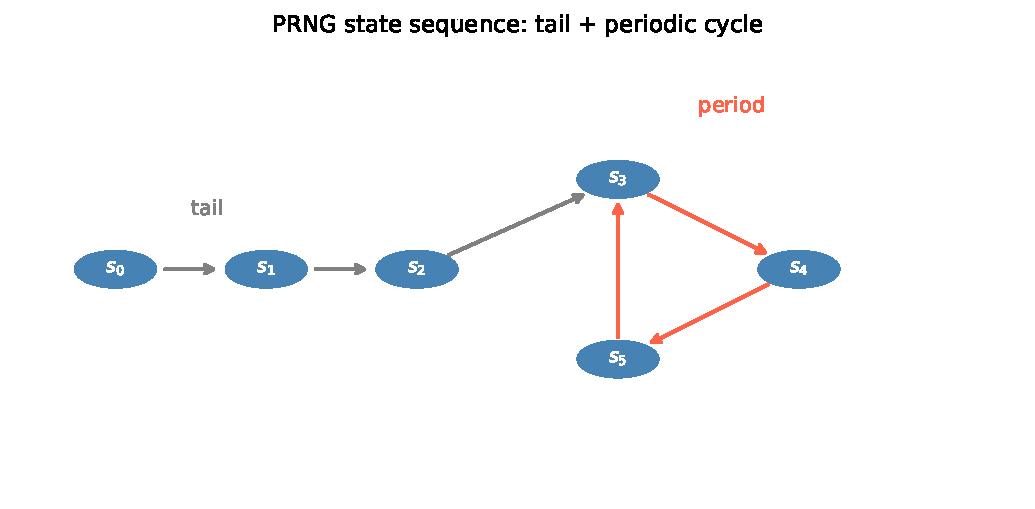
\includegraphics[width=0.52\textwidth]{prng_period}
\end{center}

The figure above illustrates the typical life-cycle of a PRNG state sequence:
there is a ``tail'' of distinct states leading into a cycle (shown as a loop),
after which the generator repeats indefinitely.  A well-designed PRNG has a
period close to $|S|$ and the tail as short as possible.

\begin{alertblock}{Key Insight: Period is Everything}
For any simulation requiring $n$ samples, the period must be much larger than
$n$.  If the period is smaller than $n$, the sequence simply starts repeating
within the simulation, producing spurious correlations that can silently
corrupt every result.  For modern simulations with $n \approx 10^9$ samples,
a period of $2^{128}$ (as in PCG64, the generator recommended throughout this
course) is essentially inexhaustible: even at $10^9$ samples per second, one
would need $10^{19}$ times the age of the universe to cycle through the entire
period once.
\end{alertblock}

\framebreak

\begin{block}{Definition 2.1.1.1 --- Three Equivalent Types of Random Sequences}

Three representations of ``random numbers'' appear throughout the literature.
They are interconvertible, and a good PRNG must simultaneously approximate all
three.

\medskip
\textbf{(i) Uniform numbers from $[0,1)$.}  We say $U_1, U_2, \ldots$ is a
sequence of random numbers from the unit interval $[0,1)$ if each $U_j$ is a
random variable with the \emph{uniform distribution} on $[0,1)$.  This means
the probability that $U_j$ falls in any sub-interval $[a,b) \subset [0,1)$
is exactly the length $b-a$ of that interval:
\[
  \mathbb{P}(U_j \le t) =
  \begin{cases} 0 & t < 0, \\ t & 0 \le t < 1, \\ 1 & t \ge 1. \end{cases}
\]
Here $\mathbb{P}(\cdot)$ (script P) denotes probability.  The shorthand
$U \sim \mathcal{U}[0,1)$ is read ``$U$ is distributed according to the
uniform distribution on $[0,1)$''.  The additional requirement that
$U_1, U_2, \ldots$ are \emph{independent and identically distributed (i.i.d.)}
means that knowing any subset of the $U_j$'s gives no information about the
others:
\[
  \mathbb{P}(U_1 \le t_1, \ldots, U_n \le t_n) = t_1 \cdot t_2 \cdots t_n,
  \quad 0 \le t_i \le 1.
\]

\textbf{(ii) Uniform random bits.}  The $B_j$ are i.i.d.\ taking values in
$\{0,1\}$ with $\mathbb{P}(B_j = 0) = \mathbb{P}(B_j = 1) = \tfrac{1}{2}$,
so every specific bit string of length $n$ has probability $1/2^n$ of
occurring.

\textbf{(iii) Uniform integers from $\bar{M}$.}  Here $\bar{M}$ is our
shorthand for the set $\{0, 1, \ldots, M-1\}$ where $M \ge 2$ is a fixed
integer.  The $Y_j$ are i.i.d.\ uniformly distributed on $\bar{M}$:
$\mathbb{P}(Y_j = k) = 1/M$ for each $k \in \bar{M}$.  We write
$Y \sim \mathcal{U}(\bar{M})$.
\end{block}

These three representations are \emph{interconvertible} by simple arithmetic.
Given a uniform number $u_i \in [0,1)$, the integer
$y_i = \lfloor M u_i \rfloor$ lies in $\bar{M}$ and is uniformly distributed.
Here $\lfloor \cdot \rfloor$ (the floor function, read ``floor of'') rounds
down to the nearest integer, so for example $\lfloor 6 \times 0.731 \rfloor
= \lfloor 4.386 \rfloor = 4$.  Conversely, $u_i = y_i / M$ recovers a
$[0,1)$ value.  Converting to bits requires care: the robust method first
converts $u_i$ to an integer $y_i$ with $M = 2^k$ and then reads the binary
digits of $y_i$, rather than using the naive threshold rule
$b_i = \mathbf{1}[u_i \ge 0.5]$ (which keeps only one bit and discards all
the rest of the precision in $u_i$ --- we explain this danger in
Section~2.5.1.1).

\medskip
The key take-away from this introduction is that a PRNG must simultaneously
approximate all three types of random sequences and must do so in a way that
survives rigorous statistical testing across many dimensions.

\end{frame}

%% ==================================================================
\begin{frame}[allowframebreaks]{2.2 Random Permutations: Shuffling and its Applications}

A \textbf{permutation} of the set $\{1, 2, \ldots, n\}$ is simply an
arrangement of its elements in some order.  For example, with $n=3$ the
possible permutations are $(1,2,3)$, $(1,3,2)$, $(2,1,3)$, $(2,3,1)$,
$(3,1,2)$, and $(3,2,1)$ --- six arrangements in total, because there are
$3! = 3 \times 2 \times 1 = 6$ ways to arrange three distinct objects.
In general, the number of permutations of $\{1,\ldots,n\}$ is
$n! = n \times (n-1) \times \cdots \times 2 \times 1$ (read ``$n$ factorial'').

A \textbf{random permutation} is one chosen \emph{uniformly at random} from
all $n!$ possible arrangements, meaning every arrangement has exactly the same
probability $1/n!$ of being selected.  Generating random permutations is a
fundamental building block of Monte Carlo algorithms.  It underlies random
shuffling of data, randomised controlled experiments (assigning treatments
to subjects), bootstrapping, and permutation-based statistical tests.

\medskip
\textbf{The naive approach and why it fails.}  One might imagine picking
elements one at a time from $\{1,\ldots,n\}$ uniformly at random, discarding
repeats until all $n$ elements have been chosen.  This is slow because later
draws must avoid an ever-growing list of already-chosen elements --- a
situation known as the \emph{coupon-collector problem}, where the expected
number of draws grows as $n \log n$.  The Fisher-Yates shuffle completely
avoids this issue by construction.

\begin{block}{Algorithm 1: Fisher-Yates Shuffle (also called the Knuth Shuffle)}

\textbf{Require:} An integer $n \ge 1$ (the number of elements to shuffle);
pseudorandom numbers $u_1, u_2, \ldots, u_n$ with each $u_i \in [0,1)$.

\textbf{Ensure:} A uniformly random permutation of $\{1, 2, \ldots, n\}$,
stored in an array $S$.

\begin{enumerate}
  \item \emph{Initialise}: set $S[i] \leftarrow i$ for $i = 1, \ldots, n$
    (begin with the identity arrangement: element $i$ sits in position $i$).
  \item \textbf{For} $i = n$ \textbf{down to} $1$ \textbf{do:}
    \begin{enumerate}
      \item Compute $k \leftarrow 1 + \lfloor i \cdot u_i \rfloor$.  This
        selects a uniformly random index $k$ from $\{1, 2, \ldots, i\}$
        (there are exactly $i$ possible values, since $\lfloor i \cdot u_i
        \rfloor \in \{0, 1, \ldots, i-1\}$).
      \item \emph{Swap} the elements at positions $k$ and $i$:
        exchange $S[k]$ and $S[i]$.
    \end{enumerate}
  \item \textbf{Return} $S$.
\end{enumerate}
\end{block}

\begin{alertblock}{How to Read This Algorithm}
At each step $i$ (counting backwards from $n$ to $1$), we pick one of the
$i$ elements currently in positions $1$ through $i$ uniformly at random and
move it into the ``final'' position $i$.  Once placed in position $i$, an
element is never touched again.  After all $n$ steps every element has been
placed exactly once, and because at each step $i$ every one of the $i$
remaining candidates is equally likely to be chosen, the overall probability
of any particular complete ordering is $\frac{1}{n} \cdot \frac{1}{n-1}
\cdots \frac{1}{1} = \frac{1}{n!}$.  The algorithm runs in exactly $n$ swap
operations, which is optimal (you cannot shuffle $n$ elements with fewer than
$n-1$ operations).
\end{alertblock}

\begin{center}
  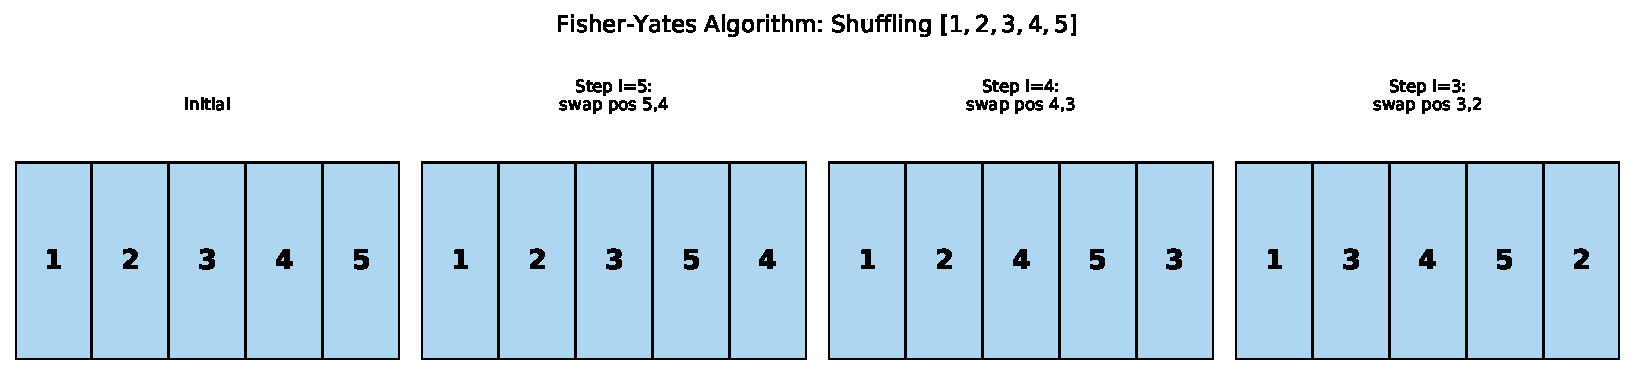
\includegraphics[width=0.78\textwidth]{fisher_yates}
\end{center}

The figure above shows a trace of Algorithm~1 for $n=5$.  At each step the
chosen element (highlighted) is swapped into its final position.  After all
five steps the resulting arrangement is guaranteed to be uniformly random.

\framebreak

\textbf{Correctness of Fisher-Yates: a rigorous inductive argument.}

We prove by induction on the loop counter $i$ that after the algorithm has
processed positions $n, n-1, \ldots, i+1$, the elements now occupying positions
$i+1, i+2, \ldots, n$ form a uniformly random arrangement of the $n-i$ elements
assigned to those positions.  This invariant guarantees that the final result
is a uniformly random permutation of all $n$ elements.

\emph{Base case} ($i = n$): At the first step, we pick a uniformly random
index $k$ from $\{1,\ldots,n\}$ and swap $S[k]$ with $S[n]$.  Every element
of $\{1,\ldots,n\}$ is equally likely to end up in position $n$, so the
element in position $n$ is uniformly distributed.  The invariant holds.

\emph{Inductive step}: Assume the elements in positions $i+1, \ldots, n$ are
already a uniformly random arrangement of their $n-i$ elements.  The $i$
elements remaining in positions $1, \ldots, i$ are therefore equally likely to
be any particular $i$-element subset of $\{1,\ldots,n\}$ not already placed.
We pick one of these $i$ remaining elements uniformly at random and move it to
position $i$.  The invariant is maintained.  After step $i=1$, every
arrangement of all $n$ elements occurs with probability $1/n!$, completing the
proof.

\begin{block}{Algorithm 2: Perm-Sort --- Generating a Random Permutation by Sorting}
An alternative approach: assign a uniformly random ``key'' to each element and
then sort by key.  The element whose key is smallest goes first, and so on.
\begin{enumerate}
  \item Initialise: $S[i] \leftarrow i$ for $i = 1,\ldots,n$.
  \item Generate $u_1,\ldots,u_n$ independently from $\mathcal{U}[0,1)$.
  \item Sort $S$ so that $u_{S[1]} \le u_{S[2]} \le \cdots \le u_{S[n]}$
    (arrange the elements so their assigned keys are in increasing order).
  \item \textbf{Return} $S$.
\end{enumerate}
\end{block}

Both algorithms produce a uniformly random permutation when given truly uniform
input.  Fisher-Yates is preferred in practice because it runs in
$\mathcal{O}(n)$ time --- one swap per step, so exactly $n$ swaps in total.
Perm-Sort requires $\mathcal{O}(n \log n)$ time for the sorting step, which is
significantly slower for large $n$.  However, Perm-Sort is sometimes easier
to parallelise because the sorting step can be distributed across multiple
processors.

\framebreak

\textbf{2.2.2 Shuffling a Deck of Cards: How Many Shuffles Are Enough?}

A standard deck of $n = 52$ cards can be identified with the set
$\{1, 2, \ldots, 52\}$.  There are $52! \approx 8.07 \times 10^{67}$ possible
orderings --- a number so fantastically large that if you shuffled a different
arrangement every second from the Big Bang until now, you would have visited
only an infinitesimally tiny fraction of all possible decks.  In practice,
this means a new physical shuffle never repeats a previous deck ordering.

A \emph{card-shuffling scheme} is a Markov chain $(X_k)_{k \ge 0}$ on the
symmetric group $\mathcal{S}_{52}$ (the mathematical name for the set of all
$52!$ permutations of 52 elements).  The chain starts in the initial ordering
$X_0 = e$ (the identity permutation) and at each step applies one random
shuffle, moving from state $X_k$ to state $X_{k+1}$.  The goal is for the
chain's distribution to converge to the \emph{uniform distribution}: every
ordering equally likely.

The distance from this ideal uniform distribution after $k$ shuffles is
measured by the \textbf{total variation distance} $d_k$ (pronounced
``dee-sub-k''):
\[
  d_k \;=\; \frac{1}{2}\sum_{\sigma \in \mathcal{S}_n}
            \left|\;\mathbb{P}(X_k = \sigma) - \frac{1}{n!}\;\right|.
\]
Here $\Sigma$ (Sigma, capital) denotes the sum over all $n!$ permutations
$\sigma$ (sigma) in $\mathcal{S}_n$.  The term inside the sum measures how
much the probability of each ordering $\sigma$ differs from the ideal uniform
probability $1/n!$.  The factor $\tfrac{1}{2}$ normalises the distance so
that $d_k \in [0,1]$.  When $d_k = 1$ the deck is in a completely predictable
(deterministic) state; when $d_k = 0$ the deck is perfectly mixed.  As more
shuffles are applied, $d_k \to 0$.

\begin{block}{How to Read the Total Variation Distance}
Think of $d_k$ as a ``percentage of remaining non-randomness''.  If $d_k =
0.5$, for example, then an adversary who could always choose the most
over-represented ordering could win a card game with probability $0.5 + 0.5 \times 0.5
= 0.75$ instead of the fair $1/n!$.  Practical applications typically aim for
$d_k < 0.01$ before considering the deck ``sufficiently shuffled''.
\end{block}

\medskip
\textbf{Common shuffling methods and their theoretical properties.}

The \emph{Top-To-Random} shuffle: remove the top card and insert it into a
uniformly random position among the $n$ available slots in the deck.  This is
the simplest scheme to analyse mathematically because the transition
probabilities are easy to compute, but it requires about $n \ln n \approx 235$
shuffles to mix a 52-card deck --- far too many for practical use.

The \emph{Riffle Shuffle (Gilbert-Shannon-Reeds model)}: cut the deck into two
halves according to a binomial distribution $\mathrm{Bin}(n, 1/2)$ (this
models the fact that in a real riffle shuffle each of the $n$ cards
independently ends up in the left or right half with equal probability), then
interleave the two halves by repeatedly dropping a card from whichever pile is
larger, with probability proportional to the current pile sizes.  This
precisely models the riffle shuffle that people perform physically at a card
table.

The \emph{Time-Reversed Riffle Shuffle}: the time-reverse of the Riffle
Shuffle interleaves two packs by independently inserting each card of one pack
into the other at a random position.  This variant is mathematically useful
because its transition probabilities have a cleaner closed form, simplifying
the analysis of mixing times.

\begin{alertblock}{The Seven-Shuffle Theorem (Bayer and Diaconis, 1992)}
For a standard 52-card deck, approximately \textbf{7 riffle shuffles} are
needed before the total variation distance $d_k$ drops below $\tfrac{1}{2}$.
With 6 shuffles the deck is still statistically far from uniformly random; with
8 it is essentially perfectly mixed.  This abrupt transition from ``unmixed''
to ``mixed'' over a small range of steps --- called the \emph{cut-off
phenomenon} --- was a landmark result in the theory of Markov chain mixing
times and has been featured in popular mathematics writing ever since.  The
proof uses Fourier analysis on the symmetric group $\mathcal{S}_{52}$ and is
one of the most elegant applications of pure mathematics to an everyday activity.
\end{alertblock}

\end{frame}

%% ==================================================================
\begin{frame}[allowframebreaks]{2.3 Pseudorandom Number Generators in Python}

Modern scientific computing in Python uses the \texttt{numpy.random} module,
which provides a carefully designed family of high-quality pseudorandom number
generators through a clean, consistent API (application programming interface).
This section describes the recommended generators, explains why they are
preferred over older alternatives, and shows how to use them in practice.

The recommended entry point for all new Python code is
\texttt{numpy.random.default\_rng(seed)}, which returns a \texttt{Generator}
object backed by the \textbf{PCG64} algorithm.  You should use this in every
Monte Carlo simulation unless you have a specific reason to do otherwise.

\begin{block}{2.3.1 The NumPy Generator Hierarchy: BitGenerators and Generators}
NumPy separates the generation of random bits from the conversion of those
bits into useful distributions.  A \emph{bit generator} (such as PCG64 or
MT19937) produces raw pseudorandom bits as fast as possible.  A \emph{generator}
(the \texttt{Generator} class) wraps a bit generator and provides methods like
\texttt{.random()}, \texttt{.integers()}, and \texttt{.permutation()} that
convert those raw bits into specific distributions.

The four main choices of bit generator are:

\begin{itemize}
  \item \textbf{PCG64} (Permuted Congruential Generator, 64-bit output): This
    is the current NumPy default.  It has a period of $2^{128}$ (approximately
    $3.4 \times 10^{38}$), passes all tests in the TestU01 BigCrush battery,
    and supports multiple independent streams via the \texttt{.advance(n)}
    method --- an essential feature for parallel simulations.  Use this unless
    you have a specific reason not to.
  \item \textbf{MT19937} (Mersenne Twister): The historically dominant
    generator, with a period of $2^{19937}-1$.  Its state space consists of
    624 integers of 32 bits each (totalling 2.5 kilobytes), making it slow to
    initialise.  It fails several tests in the TestU01 BigCrush battery,
    cannot generate independent parallel streams, and is not suitable for
    cryptographic use.  It remains the default in Python's built-in
    \texttt{random} module and in legacy NumPy code (\texttt{np.random.seed}).
  \item \textbf{Philox}: A counter-based generator based on a reduced-round
    block cipher.  It provides provably independent parallel streams by
    construction, which makes it ideal for highly parallel simulations.
  \item \textbf{SFC64} (Small Fast Counting generator, 64-bit): A very fast
    non-linear generator with a period of approximately $2^{255}$ and good
    statistical properties, useful when raw speed is the priority.
\end{itemize}
\end{block}

\textbf{Why PCG64 instead of MT19937?}

The Mersenne Twister's period of $2^{19937}-1$ is so large that it sounds
impressive, but a very long period alone does not guarantee good statistical
quality.  The Mersenne Twister fails several tests in the BigCrush battery
because its output has subtle lattice structure in high dimensions (analogous
to the lattice structure of LCGs that we study in Section~2.4).  Additionally,
its large internal state of 624 integers means it is slow to initialise and
has poor cache performance on modern CPUs.

PCG64's period of $2^{128}$, while smaller in exponent, is still
inexhaustible for any practical simulation.  More importantly, PCG64
eliminates lattice structure through a carefully designed \emph{nonlinear
output permutation} applied to the raw state, which is the reason it passes
BigCrush while MT19937 does not.

\begin{center}
  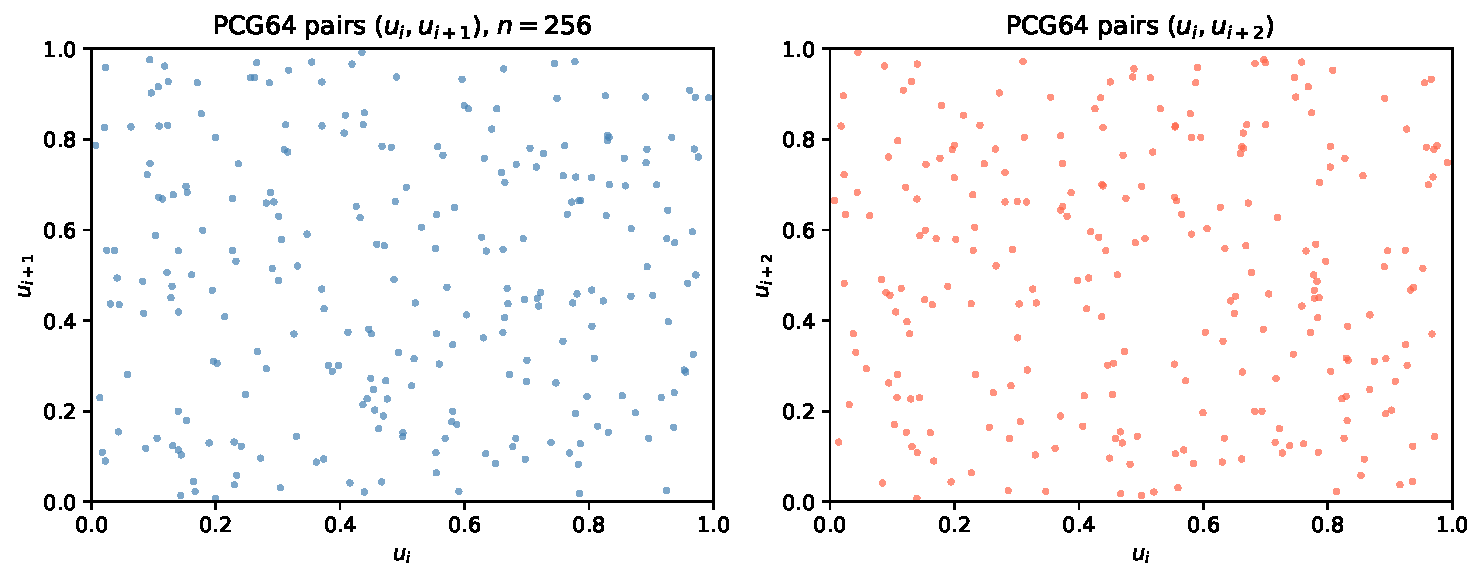
\includegraphics[width=0.52\textwidth]{pcg64_pairs}
\end{center}

The figure above shows $10{,}000$ consecutive pairs $(u_i, u_{i+1})$ produced
by PCG64.  The points fill the unit square $[0,1)^2$ densely and visually
uniformly, with no discernible structure.  This should be contrasted with the
lattice patterns visible in pairs from simple linear congruential generators
(Section~2.4), where all points lie on a small number of parallel lines.

\framebreak

\begin{block}{Converting Between Output Types in Practice}
The three output types (uniform real numbers, uniform integers, random bits)
are interconverted by the following formulas.

Given a uniform number $u_i \in [0,1)$ from the generator, conversion to an
integer $y_i \in \{0, 1, \ldots, M-1\}$ uses the floor function:
\[
  y_i \;=\; \lfloor M\, u_i \rfloor.
\]
Here $\lfloor M u_i \rfloor$ (read ``floor of $M$ times $u_i$'') rounds
$M u_i$ down to the nearest integer.  For example, if $u_i = 0.731$ and
$M = 6$ (say, for rolling a six-sided die), then
$y_i = \lfloor 6 \times 0.731 \rfloor = \lfloor 4.386 \rfloor = 4$.
The result $y_i$ is uniformly distributed on $\{0,1,\ldots,M-1\}$ whenever
$u_i$ is uniform on $[0,1)$.

The inverse: given $y_i \in \{0,\ldots,M-1\}$, the value $u_i = y_i/M$
lies in $[0,1)$ and is uniform.
\end{block}

\begin{alertblock}{Why the Naive Bit-Extraction Rule Is Dangerous}
To obtain random bits from a uniform float $u_i$, one might try the simple
threshold rule: set $b_i = 1$ if $u_i \ge 0.5$ and $b_i = 0$ otherwise.
This rule extracts only the \emph{single most significant bit} of $u_i$ and
discards all the remaining bits of precision.  A badly designed generator
that always sets the lower-order bits to zero would pass this threshold test
perfectly while being hopelessly non-random.  The correct approach is to first
convert $u_i$ to an integer $y_i = \lfloor 2^k u_i \rfloor \in \{0,\ldots,
2^k-1\}$ and then read out the $k$ binary digits of $y_i$.  NumPy's
\texttt{.integers(0, 2, size=n)} method does this correctly internally.
\end{alertblock}

\end{frame}

%% ------------------------------------------------------------------
\begin{frame}[fragile]{2.3.1 Python Code: Using NumPy PRNGs}

\begin{lstlisting}[style=python]
import numpy as np
from numpy.random import PCG64, MT19937, Generator

# --- Recommended: PCG64 via default_rng ----------------------------
# Create a Generator backed by PCG64, seeded at 42 for reproducibility.
# Changing the seed gives a completely different sequence.
rng = np.random.default_rng(seed=42)

u    = rng.random(10)           # 10 uniform numbers in [0, 1)
y    = rng.integers(0, 10, 10)  # 10 integers in {0, 1, ..., 9}
perm = rng.permutation(52)      # random permutation of {0,...,51}
print("Uniform:", u[:5])
print("Integers:", y[:5])
print("Permutation (first 8):", perm[:8], "...")

# --- Explicitly choose the bit generator --------------------------------
# Both lines below produce a Generator, but backed by different algorithms.
rng_pcg = Generator(PCG64(seed=0))
rng_mt  = Generator(MT19937(seed=0))
print("PCG64:  ", rng_pcg.random(5))
print("MT19937:", rng_mt.random(5))
# Note: the two sequences are completely different despite the same seed=0,
# because the underlying algorithms differ.

# --- Multiple independent streams (PCG64 advance) ------------------
# For parallel simulations, we need streams that are statistically
# independent of each other. We achieve this by "advancing" the
# internal state of the second stream by 2^64 steps so it starts
# from a completely different part of the period.
bg1 = PCG64(seed=0)
bg2 = PCG64(seed=0)
bg2.advance(2**64)          # jump ahead 2^64 steps in O(log n) time
rng1 = Generator(bg1)
rng2 = Generator(bg2)
print("Stream 1:", rng1.random(3))
print("Stream 2:", rng2.random(3))  # statistically independent of stream 1
\end{lstlisting}

\end{frame}

%% ------------------------------------------------------------------
\begin{frame}[allowframebreaks]{2.3.2 Cryptographic PRNGs and RC4}

For \emph{cryptographic} applications (generating encryption keys, producing
nonces for authentication protocols, etc.), passing statistical tests is
necessary but not sufficient.  A \textbf{cryptographic PRNG (CSPRNG)} must
satisfy a much stronger requirement: it must be \emph{computationally
unpredictable}.  This means that even if an adversary observes a very long
prefix of the output stream, no efficient algorithm should be able to predict
the next bit with probability significantly better than $\tfrac{1}{2}$ (the
chance of a random guess).

\medskip
\textbf{Why statistical testing alone is not enough for security.}  A test
battery such as TestU01 checks whether the output \emph{looks} uniform and
independent: whether it passes every test a statistician might apply.  But it
says nothing about whether an adversary could recover the generator's internal
state from the output.  If the state can be recovered, the adversary can
compute every past and future output value, breaking any security guarantee
entirely.  CSPRNGs close this gap by requiring that state recovery be
computationally infeasible under standard mathematical hardness assumptions.

\medskip
\textbf{RC4 (Rivest Cipher 4)} was designed by Ron Rivest in 1987 and became
the workhorse of early internet security because of its extreme simplicity and
speed.  For many years it was used in SSL/TLS (the protocol protecting web
traffic), WEP (wireless network encryption), and PDF file encryption.  RC4
operates by maintaining a permutation $S$ of $\{0, 1, \ldots, n-1\}$ (with
$n = 256$ in standard use, so the permutation has $256!$ possible states) and
generating one output byte per step.  It consists of two phases:

\begin{itemize}
  \item \textbf{Key-Scheduling Algorithm (KSA)}: Initialises the permutation
    $S$ by mixing in the secret key $K$.  This transforms the identity
    permutation into a pseudorandom permutation that depends on the key.
  \item \textbf{Pseudo-Random Generation Algorithm (PRGA)}: Streams output
    bytes by continuously updating and querying the permutation.  The
    permutation evolves with every byte produced, so the internal state is
    never static.
\end{itemize}

\framebreak

\begin{block}{Algorithm 3: RC4 Key-Scheduling Algorithm (KSA)}
\textbf{Require:} Integer $n$ (typically 256 for byte-level RC4);
key bytes $K[0], K[1], \ldots, K[L-1]$ where $L$ is the key length
(for example, $L = 16$ bytes for a 128-bit key).

\textbf{Ensure:} A pseudorandom permutation $S[0], S[1], \ldots, S[n-1]$
of $\{0,1,\ldots,n-1\}$ that depends on the key.

\begin{enumerate}
  \item \emph{Initialise}: $S[i] \leftarrow i$ for $i = 0, 1, \ldots, n-1$
    (start with the identity permutation, where each position $i$ holds the
    value $i$).
  \item Set $j \leftarrow 0$ (initialise a running index to zero).
  \item \textbf{For} $i = 0$ \textbf{to} $n-1$ \textbf{do:}
    \begin{enumerate}
      \item $j \leftarrow (j + S[i] + K[i \bmod L]) \bmod n$ \\
        (update $j$ using the current state value $S[i]$ and the key byte
        $K[i \bmod L]$; the notation $i \bmod L$ means the remainder when
        $i$ is divided by $L$, so the key ``wraps around'' if it is shorter
        than $n$).
      \item \textbf{Swap} $S[i]$ and $S[j]$.
    \end{enumerate}
  \item Reset $i \leftarrow 0$, $j \leftarrow 0$ (prepare for the PRGA phase).
\end{enumerate}

The effect of the KSA is that the key byte $K[i \bmod L]$ influences the
swap at every position $i$, mixing the key throughout the entire permutation.
Different keys produce different permutations, so the output stream is
key-dependent.
\end{block}

\begin{block}{Algorithm 4: RC4 Pseudo-Random Generation Algorithm (PRGA)}
\textbf{Require:} Permutation $S$ produced by the KSA; two counters
$i = 0$ and $j = 0$; an output-step counter $r = 0$.

\textbf{Ensure:} A stream of pseudorandom output bytes $x_0, x_1, x_2, \ldots$

\textbf{While} generating output \textbf{do:}
\begin{enumerate}
  \item $i \leftarrow (i + 1) \bmod n$
    \quad (advance the first counter by 1, wrapping around modulo $n$).
  \item $j \leftarrow (j + S[i]) \bmod n$
    \quad (advance the second counter by the current state value at $i$).
  \item \textbf{Swap} $S[i]$ and $S[j]$
    \quad (update the permutation).
  \item $x_r \leftarrow S[\,(S[i] + S[j]) \bmod n\,]$
    \quad (look up the output byte as $S$ evaluated at the sum of the two
    swapped values, modulo $n$).
  \item $r \leftarrow r + 1$.
\end{enumerate}

Each output byte $x_r$ depends on both $S[i]$ and $S[j]$ through the double
lookup, ensuring that the output is sensitive to the evolving permutation
state and not easily predictable from any single position.
\end{block}

\framebreak

\begin{center}
  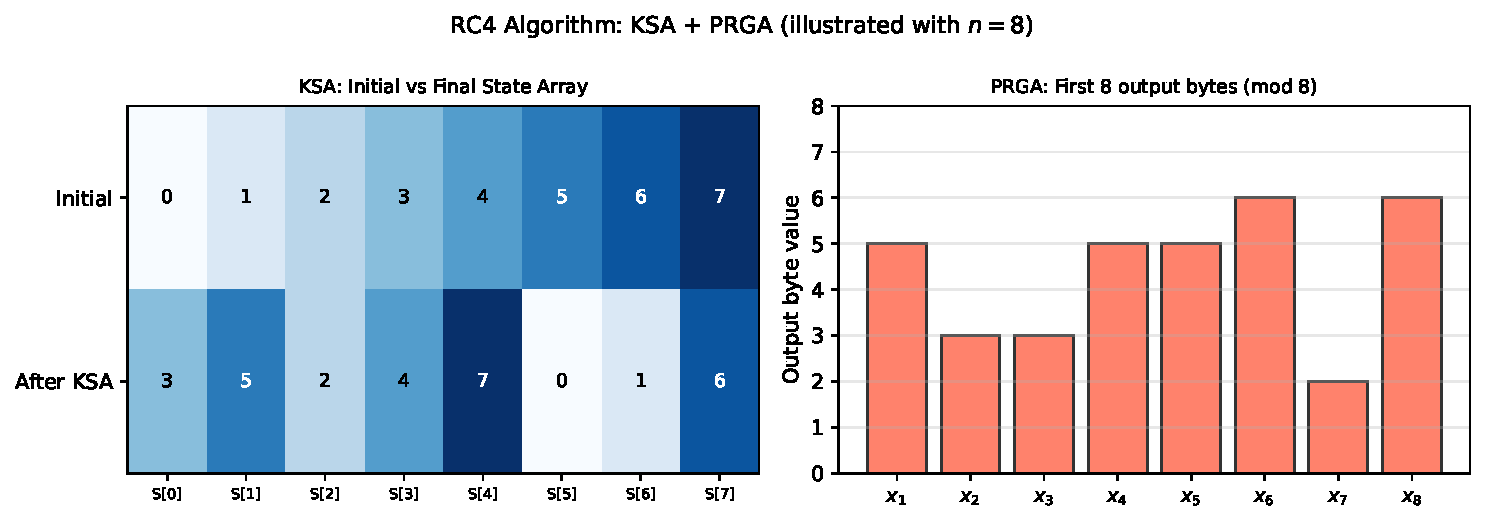
\includegraphics[width=0.62\textwidth]{rc4_schematic}
\end{center}

The figure above illustrates the KSA (left panel) and PRGA (right panel) of
RC4.  In the KSA, the key byte $K[i \bmod L]$ contributes to the running
index $j$ at each step, folding the secret key throughout the initial
permutation.  In the PRGA, both counters $i$ and $j$ advance on every step,
ensuring that every position in the permutation eventually participates in
producing output.

\medskip
\textbf{Why RC4 was eventually broken and deprecated.}

Despite its elegant design, RC4 has serious statistical biases.  The first
few hundred output bytes are statistically correlated with the secret key ---
a structural weakness.  In 2001, Fluhrer, Mantin, and Shamir showed that
WEP's practice of deriving the RC4 initialisation key from a known
initialisation vector allowed full key recovery by observing the first few
bytes of many encrypted messages (a \emph{related-key attack}).  This
vulnerability led directly to the widespread breaking of WEP-protected
wireless networks.  The IETF deprecated RC4 in RFC~7465 (February 2015),
prohibiting its use in TLS.  Modern protocols use AES in counter mode
(AES-CTR) or the ChaCha20 stream cipher, both of which have formal security
proofs under standard hardness assumptions and no known practical weaknesses.

\begin{alertblock}{Key Insight: Statistical Correctness is Not Security}
RC4 illustrates an important lesson: a generator can produce output that looks
perfectly random under standard statistical tests while still being
cryptographically broken.  For \emph{cryptographic} use, security must be
\emph{provably reducible} to a well-studied hard computational problem such as
integer factorisation or discrete logarithm.  For non-cryptographic Monte
Carlo simulation, PCG64 or MT19937 are entirely sufficient --- unpredictability
from an adversary is simply not the concern in that context.
\end{alertblock}

\end{frame}

%% ------------------------------------------------------------------
\begin{frame}[fragile]{2.3.2 Python Code: RC4 Implementation}

\begin{lstlisting}[style=python]
def rc4_ksa(n, key):
    """
    Key-Scheduling Algorithm (KSA).
    n   : state size (use 256 for standard RC4)
    key : list of integers in {0,...,n-1} (the secret key bytes)
    Returns: permutation S[0..n-1] initialised from the key.
    """
    S = list(range(n))   # start with the identity permutation
    j, L = 0, len(key)
    for i in range(n):
        # Mix in one key byte at each step.
        # i % L wraps around if the key is shorter than n.
        j = (j + S[i] + key[i % L]) % n
        S[i], S[j] = S[j], S[i]    # swap
    return S

def rc4_prga(S, num_bytes):
    """
    Pseudo-Random Generation Algorithm (PRGA).
    S         : permutation from KSA (modified in place)
    num_bytes : how many output bytes to generate
    Returns: list of pseudorandom integers in {0,...,n-1}.
    """
    n, i, j = len(S), 0, 0
    output = []
    while len(output) < num_bytes:
        i = (i + 1) % n               # advance counter i
        j = (j + S[i]) % n            # advance counter j
        S[i], S[j] = S[j], S[i]       # swap
        t = (S[i] + S[j]) % n         # lookup index
        output.append(S[t])            # output byte
    return output

# --- Example: n=256 (standard byte-level RC4), short key ---
key    = [3, 1, 4, 1, 5, 9]          # 6-byte key
S      = rc4_ksa(256, key)
stream = rc4_prga(S, 20)
print("RC4 keystream (first 20 bytes):", stream)

# IMPORTANT: In real applications, always discard the first 256 or
# more output bytes before use, because they are statistically biased
# (correlated with the key). This mitigation is known as "RC4-drop[N]".
# However, RC4 is deprecated in all modern protocols --- use ChaCha20
# or AES-CTR for any cryptographic application.
\end{lstlisting}

\end{frame}

%% ==================================================================
%%  CHAPTER 2 — SECOND HALF
%%  Sections 2.4 through 2.7 (Exercises) and the Summary frame.
%%  Reader-friendly style: full sentences, Greek pronunciation on first
%%  use per frame, Notation blocks after every formula, worked numerics.
%%  Start directly with the first \begin{frame} — no preamble.
%% ==================================================================

%% ==================================================================
\begin{frame}[allowframebreaks]{2.4 Simple Generators: Historical Perspective}

Before modern high-quality generators such as PCG64 were developed,
practitioners relied on a family of simple, mathematically transparent
generators.  These are now primarily of historical and educational interest,
but studying them in detail is the fastest way to understand \emph{why}
modern generators are designed the way they are --- and what goes wrong when
designers cut corners.

\medskip
\textbf{The fundamental challenge: lattice structure.}
Consider the linear congruential generator (LCG) with the recurrence
$x_j = (137\,x_{j-1} + 187) \bmod 256$.  This generator has a state space
of exactly 256 values, so it can at most produce 256 distinct outputs before
repeating.  If we plot all 256 consecutive pairs $(u_i,\, u_{i+1})$, where
$u_i = x_i/256$, we find that the points do \emph{not} fill the unit square
uniformly.  Instead, every single point lies on one of a small number of
parallel diagonal lines.  This is the \textbf{lattice structure} inherent
in all LCGs, and it is immediately visible to the naked eye.

\begin{center}
  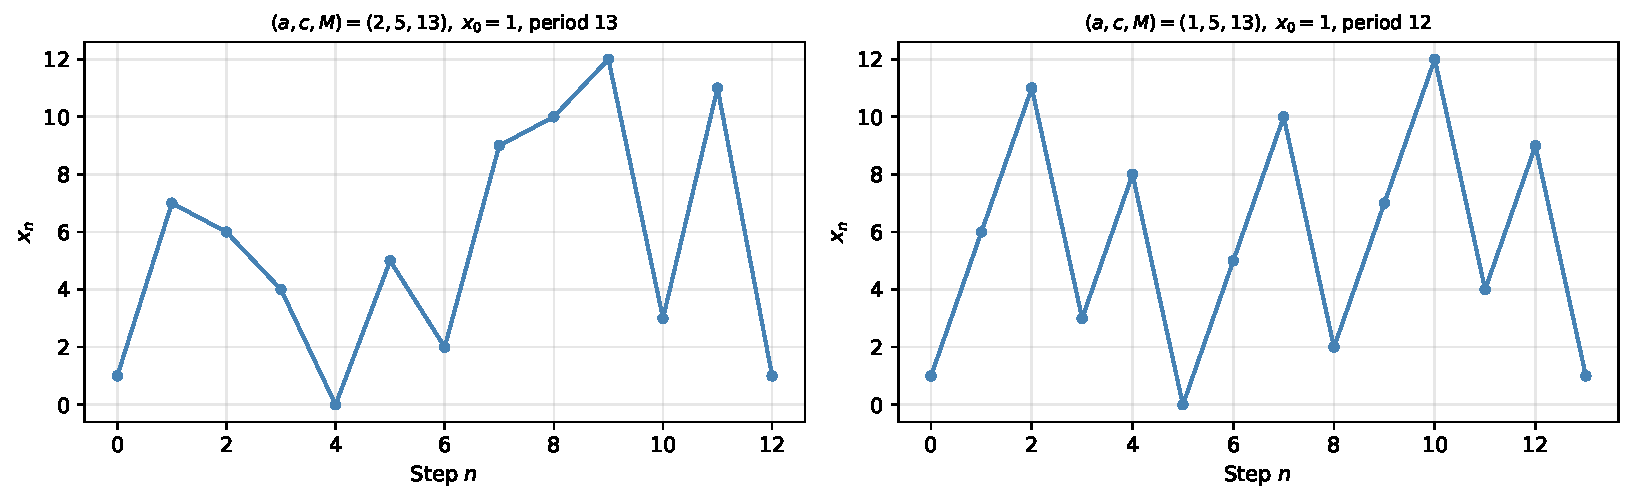
\includegraphics[width=0.80\textwidth]{lcg_sequences}
\end{center}

The figure above shows consecutive pairs $(u_i, u_{i+1})$ for a small LCG
(left panel) and a somewhat larger one (right panel).  In both cases, the
parallel-line pattern is unmistakable.  Any simulation that uses two or
more consecutive numbers from such a generator to form a two-dimensional
sample point will produce results that reflect this artificial regularity
rather than genuine randomness.  For example, a two-dimensional integral
estimated by such pairs will systematically miss the regions between the
lines, introducing a bias that does not decrease with sample size in the
usual way.

\begin{alertblock}{Key Insight: Lattice Structure Is Invisible in 1D but Fatal in Higher Dimensions}
The lattice structure of an LCG is completely invisible when numbers are
examined one at a time: the 1D marginal distribution is uniform.  It only
becomes apparent when consecutive numbers are grouped into pairs, triples,
or higher-dimensional vectors.  This is why multi-dimensional statistical
tests (Section~2.5) are essential: a generator can look perfect in 1D while
being catastrophically wrong in 2D.
\end{alertblock}

\end{frame}

%% ------------------------------------------------------------------
\begin{frame}[allowframebreaks]{2.4.1 Linear Congruential Generators (LCG)}

The \textbf{linear congruential generator (LCG)} is the simplest useful
pseudorandom number generator.  It produces a sequence of integers by
applying a linear function modulo a large integer, and its appeal is
minimal computational cost: one multiplication, one addition, and one
modulo operation per step.  An enormous body of theoretical work has been
done on LCGs, making them the best-understood generators in existence.

\begin{block}{The Linear Congruential Recurrence}
The LCG produces a sequence $x_0, x_1, x_2, \ldots$ according to:
\[
  x_{n+1} \;=\; (\,a \cdot x_n \;+\; c\,) \bmod M.
\]
This formula says: to get the next state $x_{n+1}$ (x subscript n-plus-one),
multiply the current state $x_n$ (x subscript n) by the multiplier $a$,
add the increment $c$, then take the remainder when dividing by the
modulus $M$.  The result always lies in $\{0, 1, \ldots, M-1\}$.
\end{block}

\begin{block}{Notation}
\begin{itemize}
  \item $M > 0$: the \textbf{modulus} --- the total number of possible
    states.  All outputs $x_n$ lie in $\{0, 1, \ldots, M-1\}$.
  \item $a$ (where $0 \le a < M$): the \textbf{multiplier} --- controls the
    step size in state space.
  \item $c$ (where $0 \le c < M$): the \textbf{increment} --- an additive
    offset that prevents the sequence from collapsing to zero.
  \item $x_0$: the \textbf{seed} --- the user-chosen starting value.
    Changing the seed produces a different sequence.
  \item $\bmod$ (modulo): the remainder after integer division.
    For example, $17 \bmod 5 = 2$ because $17 = 3 \times 5 + 2$.
  \item The \textbf{output} at step $n$ is $u_n = x_n / M$, which lies
    in $[0,1)$.
\end{itemize}
When $c = 0$, the generator is called a \textbf{linear multiplicative
congruential generator (LMCG)}.
\end{block}

\begin{alertblock}{How to Read This Formula}
At each step, the sequence ``jumps'' by a fixed linear rule and wraps
around at $M$.  If $M$ is large and the parameters are chosen well, the
sequence visits every value in $\{0,\ldots,M-1\}$ exactly once before
repeating --- achieving the maximum possible period of $M$.  If the
parameters are chosen poorly, the sequence may cycle through only a tiny
fraction of states, producing highly correlated outputs and a useless
generator.
\end{alertblock}

\framebreak

\begin{block}{Theorem 2.4.1 --- Full-Period Conditions (Knuth)}
Let $b = a - 1$.  The LCG has period \emph{exactly} $M$ (i.e., visits
every state in $\{0,\ldots,M-1\}$ before repeating) if and only if all
three conditions hold simultaneously:
\begin{enumerate}
  \item $\gcd(c, M) = 1$: the increment $c$ and the modulus $M$ are
    coprime, meaning they share no common integer factor other than 1.
  \item $b = a - 1$ is divisible by every prime $p$ that divides $M$.
    Recall that a prime is a number greater than 1 whose only divisors are
    1 and itself (2, 3, 5, 7, 11, $\ldots$).
  \item If $4$ divides $M$, then $4$ also divides $b$.  Equivalently:
    $a \equiv 1 \pmod{4}$, meaning the remainder of $a$ when divided by
    4 is equal to 1.
\end{enumerate}
\end{block}

\textbf{Intuition behind the conditions.}
Condition~1 ensures the increment does not create a common factor that
restricts the sequence to a proper subset of states.  For example, if
$c = 4$ and $M = 8$, then $\gcd(4,8)=4 \ne 1$, and the sequence can only
visit even states.  Condition~2 ensures that the multiplier ``rotates
through'' all residue classes.  Condition~3 is a technical correction needed
when $M$ is divisible by a high power of 2, because multiplication behaves
differently modulo powers of 2.

\begin{exampleblock}{Worked Example 2.4.2: Classical 32-bit LCG}
Choose $M = 2^{31}-1 = 2{,}147{,}483{,}647$.  This particular number is a
Mersenne prime (a prime of the form $2^p - 1$), meaning it has no divisors
other than 1 and itself.  Choose the multiplier $a = 7^5 = 16{,}807$ and
increment $c = 0$ (so this is an LMCG).

Since $M$ is prime, the full-period condition for the LMCG is simply that
$a$ is a \emph{primitive root} modulo $M$, and $16{,}807 = 7^5$ satisfies
this.  The period is $M - 1 = 2{,}147{,}483{,}646 \approx 2.1 \times 10^9$.
This was among the most widely used generators for 32-bit computers and was
proposed by Lewis, Goodman, and Miller.  Other well-known choices include
$a = 40{,}014$ with the same $M$, and for 36-bit machines: $M = 2^{35}-31$,
$a = 5^5 = 3{,}125$.
\end{exampleblock}

\begin{exampleblock}{Worked Example 2.4.3: Small LCG (Resing's Example)}
Take $(a, c, M) = (1, 5, 13)$ with seed $x_0 = 1$.

\textbf{Step 1 --- verify full-period conditions:}
$b = a - 1 = 0$.  Since $M = 13$ is prime, its only prime divisor is 13,
and $13 \mid 0$ (13 divides 0) trivially.  Also $\gcd(5, 13) = 1$ since
$5 < 13$ and both are prime.  Condition~3 is irrelevant because $4 \nmid 13$.
All conditions are satisfied, so the period is $M = 13$.

\textbf{Step 2 --- trace the sequence from $x_0 = 1$:}
\[
  1 \;\to\; 6 \;\to\; 11 \;\to\; 3 \;\to\; 8 \;\to\; 0 \;\to\; 5
  \;\to\; 10 \;\to\; 2 \;\to\; 7 \;\to\; 12 \;\to\; 4 \;\to\; 9
  \;\to\; 1 \;\to\; \cdots
\]
(Check the first step: $(1 \times 1 + 5) \bmod 13 = 6 \bmod 13 = 6$.
Second step: $(1 \times 6 + 5) \bmod 13 = 11$. Third: $(11+5)\bmod 13 = 3$.
And so on.)  The sequence visits all 13 values $\{0, 1, \ldots, 12\}$
exactly once before returning to 1 --- confirming period 13.

\textbf{Counter-example:} Take $(a, c, M) = (2, 5, 13)$ with $x_0 = 1$.
Now $b = a - 1 = 1$.  We need every prime dividing $M=13$ to also divide $b=1$.
But $13 \nmid 1$ (13 does not divide 1), so condition~2 fails.  Indeed, the
period is only 12, not 13.  Moreover, starting from $x_0 = 8$ gives the
constant sequence $8 \to 8 \to 8 \to \cdots$ with period 1 --- a completely
degenerate generator.
\end{exampleblock}

\framebreak

\begin{center}
  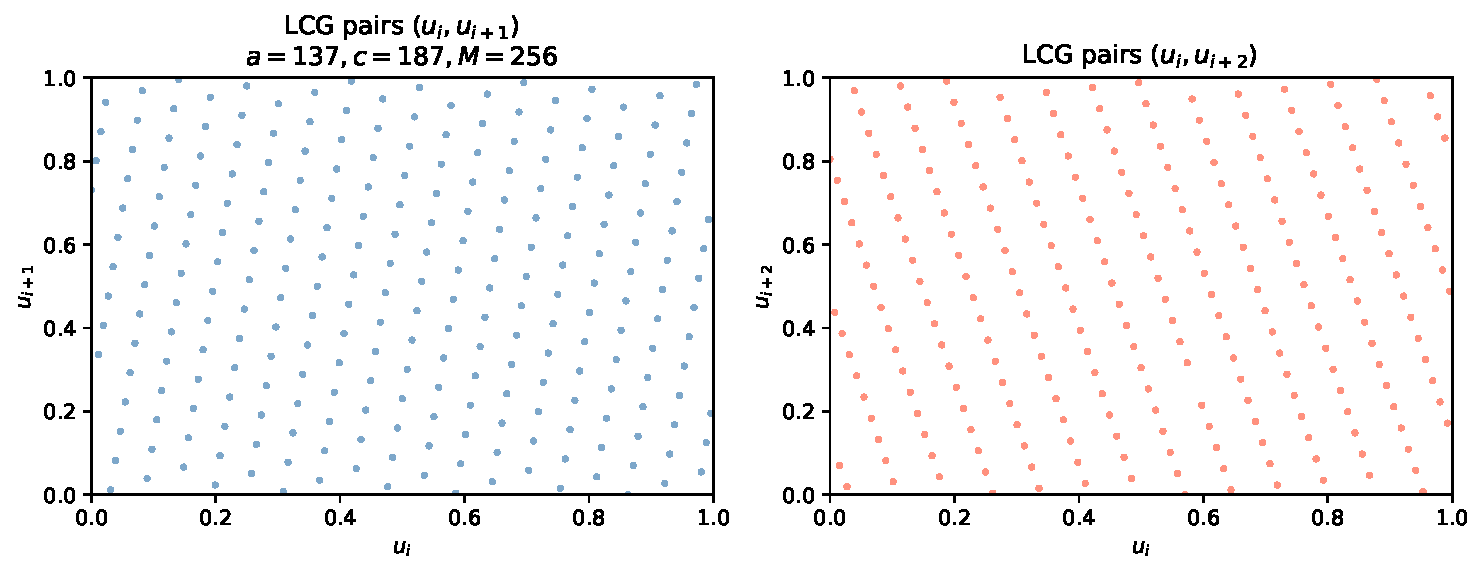
\includegraphics[width=0.82\textwidth]{lcg_pairs}
\end{center}

The figure shows $(u_i, u_{i+1})$ pairs for a small-state LCG.  The lattice
structure --- all points lying on a small number of parallel lines rather than
filling the square uniformly --- is unmistakable.  This lattice structure is
not an accident: it is an inevitable consequence of the linear arithmetic,
described precisely by the following theorem.

\begin{block}{Marsaglia's Theorem (1968)}
The $d$-dimensional (d is a positive integer indicating how many consecutive
outputs are grouped together) vectors
$(u_i,\, u_{i+1},\, \ldots,\, u_{i+d-1})$ produced by \emph{any} LCG
with modulus $M$ always lie on a grid of parallel hyperplanes
(flat, $(d-1)$-dimensional subspaces of $d$-dimensional space).
The number of such hyperplanes is at most $M^{1/d}$.
\end{block}

\begin{block}{Notation for Marsaglia's Theorem}
\begin{itemize}
  \item $d$: the dimension (number of consecutive outputs grouped
    together).
  \item $M^{1/d}$ (M to the power one-over-d): the $d$-th root of $M$.
    For example, if $M = 10^9$ and $d = 3$, then $M^{1/3} = 10^3 = 1000$
    hyperplanes at most.
  \item A \textbf{hyperplane} in $d$ dimensions is the
    $(d-1)$-dimensional analogue of a line (in 2D) or a plane (in 3D).
    In 2D, it is a line; in 3D, it is a plane.
\end{itemize}
\end{block}

\begin{alertblock}{How to Read Marsaglia's Theorem}
The theorem says that no matter how large $M$ is, in higher dimensions the
lattice structure \emph{always} appears.  As $d$ increases, $M^{1/d}$
decreases: for $M = 2^{31}$ and $d = 6$, the bound is only
$(2^{31})^{1/6} \approx 2^{5.2} \approx 37$ hyperplanes.  This means a
simulation that uses 6-dimensional samples from an LCG might see all its
points concentrated on just 37 parallel planes --- a catastrophic lack of
coverage.  This is why LCGs are unsuitable for high-dimensional Monte Carlo.
\end{alertblock}

\framebreak

\textbf{Commercial LCG parameters historically used in widely distributed software.}

\medskip
The table below lists the exact recurrences used in popular software.  Each
was chosen for implementation simplicity or speed on the hardware of its era.
By modern standards, all of them fail the TestU01 BigCrush test battery.

\medskip
\begin{center}
\begin{tabular}{lll}
  \toprule
  System & Recurrence & Output formula \\
  \midrule
  \textbf{Java} &
    $x_{i+1} = (25{,}214{,}903{,}917\,x_i + 11) \bmod 2^{48}$ &
    $u_i = \bigl(2^{27}\lfloor x_{2i}/2^{22}\rfloor
           + \lfloor x_{2i+1}/2^{21}\rfloor\bigr)/2^{53}$ \\[3pt]
  \textbf{rand48 (UNIX)} &
    same $x_i$ recurrence as Java &
    $u_i = x_i / 2^{48}$ \\[3pt]
  \textbf{Visual Basic} &
    $x_i = (1{,}140{,}671{,}485\,x_{i-1} + 12{,}820{,}163) \bmod 2^{24}$ &
    $u_i = x_i / 2^{24}$ \\[3pt]
  \textbf{Excel} &
    $u_i = (0.9821\,u_{i-1} + 0.211327) \bmod 1$ & direct \\
  \bottomrule
\end{tabular}
\end{center}

\medskip
The Java formula is particularly instructive: it takes the high bits from two
consecutive LCG states and combines them to form a 53-bit double-precision
float.  This trick improves the 1D output quality but does not fix the
2D lattice structure.

\framebreak

\textbf{Generalisations of the linear congruential method.}

The \textbf{generalised linear congruential generator (GLCG)} extends the
basic recurrence to use the $k$ (k is a positive integer, the \emph{order}
of the recurrence) most recent states:
\[
  x_n \;=\; \bigl(a_1\,x_{n-1} \;+\; a_2\,x_{n-2} \;+\; \cdots
             \;+\; a_k\,x_{n-k} \;+\; c\bigr) \bmod M.
\]

\begin{block}{Notation}
\begin{itemize}
  \item $k$: the \textbf{order} --- how many past states feed into the
    next state.  The ordinary LCG has $k=1$.
  \item $a_1, a_2, \ldots, a_k$: the \textbf{coefficients} --- weights
    on each past state.
  \item $c$: the \textbf{increment} (same as before).
  \item $M$: the \textbf{modulus} (same as before).
\end{itemize}
When $M$ is prime and the \emph{characteristic polynomial}
$p(\lambda) = \lambda^k - a_1\lambda^{k-1} - \cdots - a_k$ is a
\textbf{primitive polynomial} over the Galois field $\mathrm{GF}(M)$
(the field with $M$ elements, where arithmetic is modulo $M$), the period
reaches the theoretical maximum of $M^k - 1$.  Here $\lambda$ (lambda)
is a placeholder variable.  For example, with $M = 2$ and $k = 32$,
the period can be $2^{32} - 1 \approx 4.3 \times 10^9$ --- far exceeding
the period of a simple LCG with the same modulus.
\end{block}

\medskip
\textbf{Quadratic and cubic generators} replace the linear recurrence with
nonlinear recurrences, which break the lattice structure at the cost of
slower arithmetic (nonlinear operations are more expensive than addition):
\begin{itemize}
  \item \emph{QCG I (Quadratic Congruential Generator, type I)}:
    $x_{i+1} = x_i^2 \bmod M$, where $M$ is a 512-bit prime.  The
    squaring operation (raising $x_i$ to the power 2) introduces nonlinearity.
  \item \emph{QCG II (type II)}: $x_{i+1} = 2x_i^2 + 3x_i + 1 \bmod 2^{512}$.
  \item \emph{CCG (Cubic Congruential Generator)}: $x_{i+1} = 2x_i^3 \bmod 2^{512}$,
    where $x_i^3$ means $x_i$ cubed (multiplied by itself twice).
\end{itemize}

\framebreak

\textbf{Fibonacci and Lagged Fibonacci Generators.}

The simplest extension of the LCG idea uses \emph{two} past states instead of
one, analogous to the Fibonacci sequence (where each number is the sum of the
two preceding ones).  The standard \textbf{lagged Fibonacci generator} is:
\[
  x_n \;=\; x_{n-k} \;+\; x_{n-l} \bmod M, \quad n \;\ge\; \max(k, l),
\]
with recommended parameters $k = 100$, $l = 37$, $M = 2^{30}$.

\begin{block}{Notation}
\begin{itemize}
  \item $k$ and $l$ (l): the two \textbf{lags} --- how far back in the
    sequence we look for the two inputs.  Choosing $k$ and $l$ far apart
    ensures the two inputs are nearly independent.
  \item $M = 2^{30}$: a power of 2 is chosen so the modulo operation can
    be implemented as a fast bitwise AND instead of integer division.
  \item The sequence requires $\max(k,l) = 100$ initial values (a seed
    of length 100) before it can start generating outputs.
\end{itemize}
The period of the lagged Fibonacci generator with these parameters is
approximately $(2^{100} - 1) \times 2^{30} \approx 2^{130}$ --- very long,
with simple arithmetic.  However, the $100$-value initialisation seed is
large and must itself be generated by a good PRNG.
\end{block}

\medskip
\textbf{L'Ecuyer Combined Generator.}
To achieve both a very long period and reduced lattice structure,
L'Ecuyer (1988) combined \emph{two} GLCG sequences.  The key observation is
that if two LCGs have different lattice structures, their combination tends
to cancel the worst features of each.  The combined output has a period
approximately equal to the \emph{product} of the two individual periods.
The generator is defined by the following four-step procedure:

\begin{enumerate}
  \item $x_n = (A_1\,x_{n-2} - A_2\,x_{n-3}) \bmod M_1$
    \hfill (first GLCG of order 2)
  \item $y_n = (B_1\,y_{n-1} - B_2\,y_{n-3}) \bmod M_2$
    \hfill (second GLCG of order 1 and 3)
  \item $z_n = (x_n - y_n) \bmod M_1$
    \hfill (combine by subtraction modulo $M_1$)
  \item Output: $u_n = z_n/(M_1+1)$ if $z_n > 0$; otherwise
    $u_n = M_1/(M_1+1)$.
    \hfill (map to $(0,1)$)
\end{enumerate}

The specific parameter values (chosen by L'Ecuyer to satisfy primitive
polynomial conditions on both moduli):
$M_1 = 4{,}294{,}967{,}087$,\ $M_2 = 4{,}294{,}944{,}443$,
$A_1 = 1{,}403{,}580$,\ $A_2 = 810{,}728$,
$B_1 = 527{,}612$,\ $B_2 = 1{,}370{,}589$.

The period of the combined generator is approximately
$M_1^2 \cdot M_2 / 2 \approx 2^{191}$, achieved from two components each
with period only $\approx 2^{32}$.  This is the combination principle at work.

\begin{alertblock}{Key Insight: Combining Imperfect Generators}
Combining two generators with different lattice structures typically yields
a better generator than either component alone, because the lattice
structures are offset and partially cancel each other.  This combination
principle is the reason L'Ecuyer's generator achieves a period of
$\approx 2^{191}$ while each component has period only $\approx 2^{32}$.
The same principle underlies all modern composite PRNGs.
\end{alertblock}

\end{frame}

%% ------------------------------------------------------------------
\begin{frame}[fragile]{2.4.1 Python Code: LCG Implementation and Lattice Visualisation}

\begin{lstlisting}[style=python]
import numpy as np
import matplotlib.pyplot as plt

def lcg(a, c, M, x0, n):
    """Linear Congruential Generator: return n uniform outputs."""
    x, seq = x0, []
    for _ in range(n):
        x = (a * x + c) % M
        seq.append(x / M)
    return seq

# Example 2.4.3: (a,c,M) = (1,5,13), x0=1 => full period 13
u = lcg(a=1, c=5, M=13, x0=1, n=14)
print("LCG (1,5,13), x0=1:", [f"{v:.3f}" for v in u])
# -> [0.462, 0.846, 0.231, 0.615, 0.000, 0.385, 0.769, ...]

# Example 2.4.3 counter-case: period only 12, not 13
u2 = lcg(a=2, c=5, M=13, x0=1, n=14)
print("LCG (2,5,13), x0=1:", [f"{v:.3f}" for v in u2])

# Visualise the lattice structure for a 256-state LCG
u256 = lcg(a=137, c=187, M=256, x0=1, n=256)
plt.figure(figsize=(5, 4))
plt.scatter(u256[:-1], u256[1:], s=4, alpha=0.7)
plt.title("LCG pairs: visible lattice structure")
plt.xlabel(r"$u_i$"); plt.ylabel(r"$u_{i+1}$")
plt.tight_layout(); plt.savefig("lcg_scatter.pdf")

def period(a, c, M, x0):
    """Find the period of an LCG by Floyd's cycle detection."""
    x, seen = x0, {}
    for k in range(10 * M):
        if x in seen:
            return k - seen[x]
        seen[x] = k
        x = (a * x + c) % M
    return None

print("Period (1,5,13):", period(1, 5, 13, 1))   # -> 13 (full)
print("Period (2,5,13):", period(2, 5, 13, 1))   # -> 12 (not full)
print("Period (2,5,13) from x0=8:", period(2, 5, 13, 8))  # -> 1
\end{lstlisting}

\end{frame}

%% ------------------------------------------------------------------
\begin{frame}[allowframebreaks]{2.4.2 Bit Generators: Building Randomness from Binary Operations}

Many pseudorandom number generators operate directly on \emph{bits} (values
of 0 or 1) rather than integers.  These \textbf{bit generators} exploit the
fact that a modern computer can perform operations on an entire 64-bit word
(a sequence of 64 binary digits stored together) in a single clock cycle.
The operations used are XOR (exclusive or) and bit shifts, both of which are
extremely fast at the hardware level.  Cryptographic generators also
inherently operate at the bit level, since encryption and decryption are
fundamentally bitwise.

\begin{block}{Fundamental Bit Operations}
\textbf{Exclusive OR (XOR)}, written $\oplus$ (read ``ex-or'' or ``XOR''):
returns 1 if and only if exactly one of its two inputs is 1.  For single
bits: $0 \oplus 0 = 0$,\ $0 \oplus 1 = 1$,\ $1 \oplus 0 = 1$,\
$1 \oplus 1 = 0$.

For multi-bit words, XOR is applied element-by-element (position by position).
Example with 4-bit words: $1011 \oplus 0110 = 1101$.

Two important properties of XOR:
\begin{enumerate}
  \item $x \oplus x = 0$ for any $x$: XOR-ing a value with itself always
    gives zero.
  \item $x \oplus 0 = x$ for any $x$: XOR-ing with zero leaves the value
    unchanged.
\end{enumerate}

\textbf{Left shift} $\ll a$ (``shift left by $a$ positions''): moves all
bits $a$ positions to the left, filling the $a$ vacated positions on the
right with zeros.  This is equivalent to multiplying by $2^a$ (2 to the
power $a$) in ordinary arithmetic, but implemented in hardware without
actual multiplication.  For example, $x \ll 2$ multiplies $x$ by 4.

\textbf{Right shift} $\gg b$ (``shift right by $b$ positions''): moves all
bits $b$ positions to the right, discarding the $b$ rightmost bits and
filling the $b$ vacated positions on the left with zeros.  This is
equivalent to integer division by $2^b$.  For example, $x \gg 3$ divides
$x$ by 8 and discards the remainder.
\end{block}

\begin{center}
  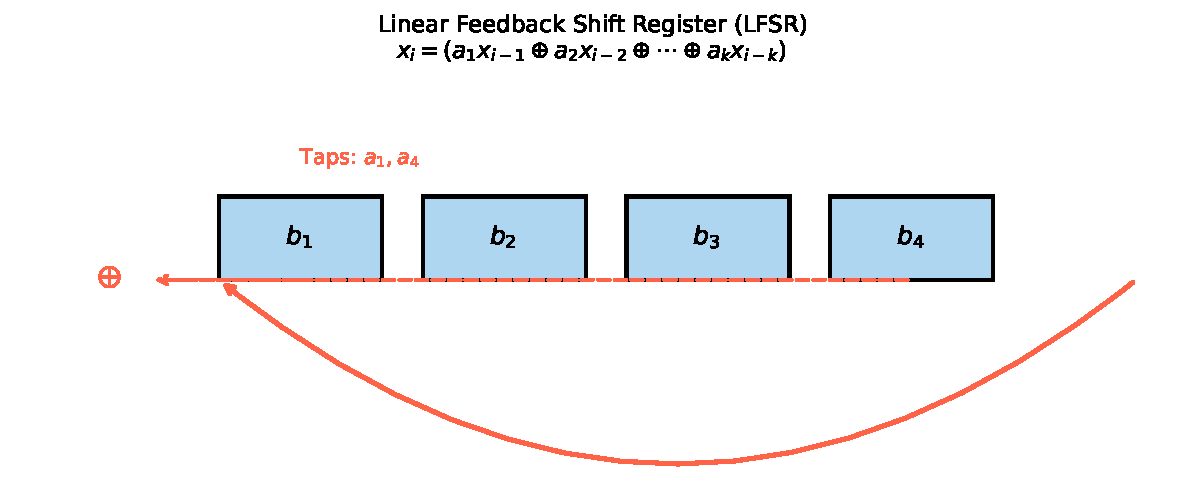
\includegraphics[width=0.62\textwidth]{lfsr_schematic}
\end{center}

The figure shows the schematic of a Linear Feedback Shift Register (LFSR).
A $k$-bit register (a sequence of $k$ storage cells, each holding one bit)
is advanced one step by shifting all bits right by one position and computing
a new leftmost bit as the XOR of selected positions (the ``taps'').

\framebreak

\begin{block}{Exclusive OR Generator (XORG)}
The XORG is one of the simplest bitwise generators, using a lag of 127 steps:
\[
  x_i \;=\; x_{i-1} \;\oplus\; x_{i-127}, \quad i \;\ge\; 128.
\]
Each new bit $x_i$ (x subscript i) is the XOR of the immediately preceding
bit $x_{i-1}$ (one step back) and the bit from 127 steps ago $x_{i-127}$.
The generator requires a 127-bit initialisation (seed) $x_1, x_2, \ldots, x_{127}$
before it can produce new bits.  The lag of 127 gives the generator memory
that prevents the trivially short cycles of a 1-step XOR recurrence.

\textbf{Worked example} (tiny version with lag 3, 4-bit seed $x_0=1, x_1=0,
x_2=1$):
$x_3 = x_2 \oplus x_0 = 1 \oplus 1 = 0$.
$x_4 = x_3 \oplus x_1 = 0 \oplus 0 = 0$.
$x_5 = x_4 \oplus x_2 = 0 \oplus 1 = 1$.
$x_6 = x_5 \oplus x_3 = 1 \oplus 0 = 1$. And so on.
\end{block}

\begin{block}{Linear Feedback Shift Register (LFSR)}
An LFSR stores $k$ bits in a shift register and computes the new bit from a
linear combination of selected positions (called \emph{taps}):
\[
  x_i \;=\; a_1\,x_{i-1} \;\oplus\; a_2\,x_{i-2} \;\oplus\; \cdots
            \;\oplus\; a_k\,x_{i-k}.
\]

\begin{itemize}
  \item $k$: the \textbf{register length} --- the number of bits stored.
  \item $a_j \in \{0,1\}$ (a subscript j): the \textbf{feedback coefficients}
    --- either 0 (meaning position $j$ does not contribute) or 1 (meaning
    it does).  The positions $j$ where $a_j = 1$ are called the \emph{taps}.
  \item The all-zeros state must be excluded: once all $k$ bits are 0, the
    LFSR produces zeros forever.
  \item When the feedback polynomial $p(z) = 1 + a_1 z + \cdots + a_k z^k$
    is a \textbf{primitive polynomial} over $\mathrm{GF}(2)$ (the field with
    just two elements, 0 and 1), the LFSR achieves the maximum period of
    $2^k - 1$.  For example, a 32-tap LFSR with the right primitive
    polynomial has period $2^{32} - 1 \approx 4.3 \times 10^9$.
\end{itemize}

\textbf{Critical weakness:} LFSRs are not cryptographically secure.  Given
any $2k$ consecutive output bits, one can recover the entire feedback
polynomial by solving a system of $2k$ linear equations over $\mathrm{GF}(2)$
(the Berlekamp-Massey algorithm).  Once the polynomial is known, all future
and past bits can be computed.  For non-cryptographic simulations, LFSRs
can be adequate, but they should never be used where security matters.
\end{block}

\framebreak

\begin{block}{Blum-Blum-Shub (BBS) Generator --- Provably Secure but Slow}
The BBS generator is the canonical example of a bit generator that is
\emph{provably} cryptographically secure under a well-established mathematical
assumption.  The recurrence is:
\[
  x_{i+1} \;=\; x_i^2 \bmod M, \quad M \;=\; p\,q,
\]
where $p$ and $q$ (q) are large distinct prime numbers both satisfying
$p \equiv q \equiv 3 \pmod{4}$ (that is, both primes leave a remainder of
3 when divided by 4).  The output at step $i$ is the \textbf{least significant
bit} (the last bit in the binary representation) of $x_i$.

\begin{itemize}
  \item $x_i^2$: $x_i$ squared (multiplied by itself).
  \item $M = p\,q$: the \textbf{modulus}, which is the product of two large
    secret primes.  Typical sizes: $p$ and $q$ are 512-bit primes, making
    $M$ a 1024-bit number.
  \item The security rests on the \textbf{quadratic residuosity assumption}:
    without knowing the factorisation $M = p\,q$, no computationally efficient
    algorithm can distinguish ``quadratic residues'' (numbers that are perfect
    squares modulo $M$) from non-residues.  This is believed to be as hard as
    factoring $M$ --- the basis of RSA cryptography.
\end{itemize}

The BBS generator is provably secure, but computing $x_i^2 \bmod M$ for a
1024-bit number $M$ requires big-integer modular multiplication, which is
about $10^5$ times slower than a single XOR operation.  This makes BBS
impractical for high-throughput Monte Carlo use.
\end{block}

\begin{block}{Shift-XOR Generator (SXR) --- Fast Practical Middle Ground}
The SXR generator combines shifts and XOR for a fast, statistically reasonable
non-cryptographic generator operating on an $n$-bit word (typically $n=32$
or $n=64$):
\begin{enumerate}
  \item Choose seed $x_0 \in \{1, \ldots, 2^n - 1\}$ (any nonzero value).
  \item Apply the recurrence:
    \[
      x_{i+1} \;=\; \bigl(x_i \;\oplus\; (x_i \ll a)\bigr)
                    \;\oplus\; (x_i \gg b),
    \]
    where $a$ and $b$ are chosen shift parameters.
  \item The output is $x_{i+1}$, interpreted as a $2^n$-valued integer.
\end{enumerate}

\textbf{Worked example} with $n=32$, $a=13$, $b=17$, seed $x_0 = 1$:
\begin{align*}
  \text{Step 1: } x_0 \ll 13 &= 2^{13} = 8192. \\
  x_0 \oplus (x_0 \ll 13) &= 1 \oplus 8192 = 8193. \\
  x_0 \gg 17 &= 0 \quad (\text{since } 1 < 2^{17}). \\
  x_1 &= 8193 \oplus 0 = 8193.
\end{align*}
From $x_1 = 8193$, the next step applies the same formula.  After a few
steps the values grow and mix, producing outputs that fill the full 32-bit
range.  The period is $2^n - 1$ when the parameters are chosen so the
characteristic polynomial is primitive over $\mathrm{GF}(2)$.
\end{block}

\begin{alertblock}{Key Insight: The Speed-Security Spectrum}
The three generators form a spectrum from fastest-but-weakest to
slowest-but-strongest.  An LFSR uses one XOR per bit and is trivially broken
by the Berlekamp-Massey algorithm.  BBS is provably secure but about $10^5$
times slower per bit.  SXR is a practical middle ground for non-cryptographic
Monte Carlo simulations: it is fast (three operations per word), produces
statistically reasonable output for most tests, and has no known simple attack,
but it lacks formal security proofs.
\end{alertblock}

\end{frame}

%% ==================================================================
\begin{frame}[allowframebreaks]{2.5 Testing Good Properties of PRNGs}

The quality of a pseudorandom number generator directly determines the
reliability of any simulation, integral estimate, or statistical analysis
built on top of it.  A generator that looks good in one dimension may fail
badly in two or more dimensions.  Statistical testing is how we gain
confidence --- before committing to a generator for a long, expensive
simulation --- that its output is \emph{indistinguishable} from truly random
output for all practical purposes.

\medskip
There are two complementary approaches to assessing PRNG quality.

\textbf{Theoretical tests} examine the internal algebraic structure of the
generator.  The most important example is the \emph{spectral test}: it
analyses the geometry of the lattice formed by the $d$-dimensional vectors
$(u_i, u_{i+1}, \ldots, u_{i+d-1})$ and measures the minimum distance
between consecutive parallel hyperplanes containing all these points.  A
large minimum distance (meaning the hyperplanes are densely and evenly
packed) indicates good $d$-dimensional uniformity.  Theoretical tests can
certify quality without running the generator at all, but they only apply
to generators whose structure is mathematically tractable.

\textbf{Statistical tests} treat the PRNG as a black box and apply
hypothesis tests to the output sequence.  The question is: could this
sequence plausibly have been produced by a truly random source?

\medskip
\textbf{Major test batteries in current use:}

\emph{Diehard} (Marsaglia): 18 tests.  Historically important but now
superseded.  Many generators that pass Diehard fail the more stringent
modern tests.

\emph{TestU01} (L'Ecuyer and Simard): three nested batteries of increasing
severity --- SmallCrush (10 tests), Crush (96 tests), BigCrush (106 tests).
BigCrush requires approximately $10^{10}$ (ten billion) random numbers to
complete one full run and is the most demanding PRNG test battery in current
use.  Any generator that fails BigCrush should not be used for serious
Monte Carlo work.

\emph{NIST SP 800-22}: 15 tests designed for cryptographic PRNGs, with
emphasis on bit-level properties.  These are the tests used by the US
government to certify random number generators for cryptographic applications.

\begin{center}
  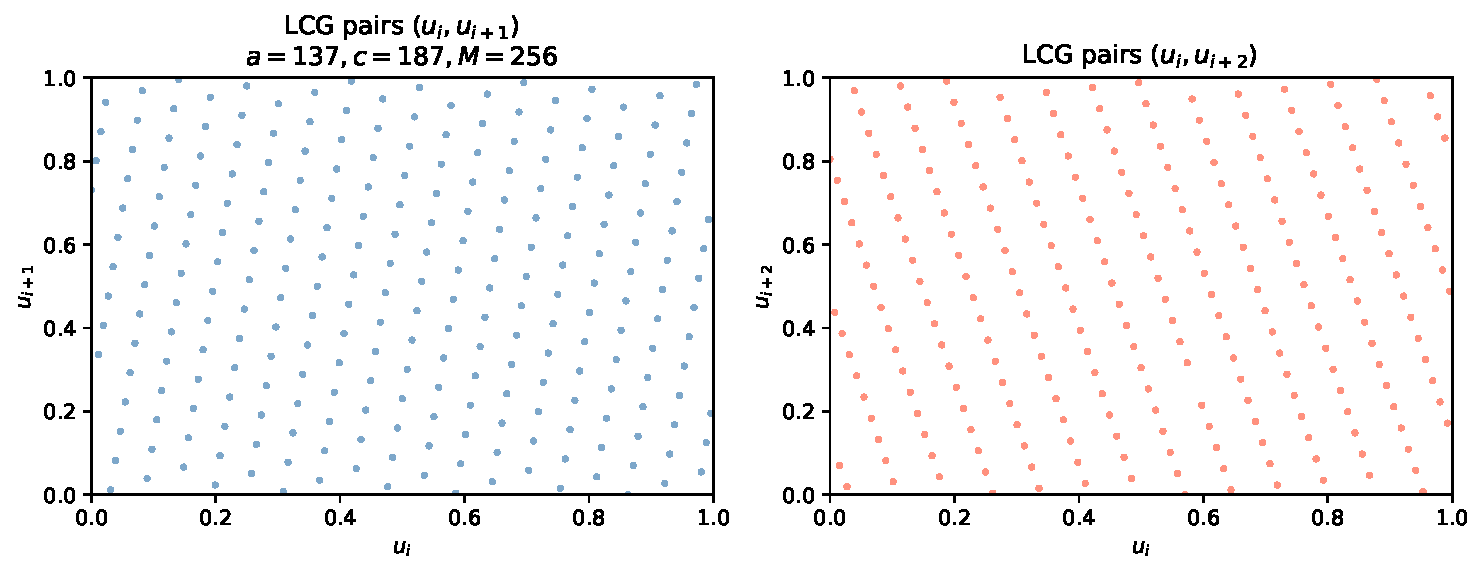
\includegraphics[width=0.82\textwidth]{lcg_pairs}
\end{center}

The figure provides a visual illustration of why testing is essential: pairs
$(u_i, u_{i+1})$ from a simple 256-state LCG lie on a few parallel lines,
immediately failing a visual test for 2D uniformity.  A good generator's
pairs should fill the square densely and uniformly.

\begin{alertblock}{Key Insight: A Test Can Only Reject, Never Confirm}
No finite set of tests can \emph{prove} that a generator is random ---
a sequence can pass every test in a battery and still be deterministic with
a known structure.  Tests can only \emph{reject} generators that are
demonstrably non-random.  Passing all tests of a respected battery (such as
TestU01 BigCrush) gives strong practical confidence but not a mathematical
guarantee.
\end{alertblock}

\end{frame}

%% ------------------------------------------------------------------
\begin{frame}[allowframebreaks]{2.5.1 Preliminary Remarks: Notation and Conversions}

Before describing specific tests, we establish notation and address two
practical matters: how to correctly convert between output formats, and
how to organise a sequence into multi-dimensional vectors for testing.

\medskip
\textbf{Standard notation.}  We use capital letters for random variables
(quantities whose values are uncertain until observed) and lowercase letters
for specific observed values (realisations):
\begin{itemize}
  \item $U \sim \mathcal{U}[0,1)$: $U$ (capital U) is a random variable
    uniformly distributed on $[0,1)$.  Its realisation (a specific observed
    value) is denoted $u$ (lowercase u).
  \item $B \sim \mathcal{U}(\{0,1\})$: $B$ is a uniform random bit (equally
    likely to be 0 or 1).  Realisation: $b$.
  \item $Y \sim \mathcal{U}(\bar{M})$: $Y$ is uniformly distributed on the
    integers $\{0, 1, \ldots, M-1\}$.  Here $\bar{M}$ (M with a bar) is
    shorthand for this set.  Realisation: $y$.
\end{itemize}

\begin{block}{2.5.1.1 Converting Between Output Formats: The Right Way and the Wrong Way}
Given a sequence $u_1, u_2, \ldots$ of values in $[0,1)$, convert to
integers in $\{0, \ldots, M-1\}$ via the floor function:
\[
  y_i \;=\; \lfloor M\,u_i \rfloor.
\]
Here $\lfloor \cdot \rfloor$ (the floor function, pronounced ``floor of'')
rounds down to the nearest integer.  For example, if $u_i = 0.731$ and
$M = 6$, then $y_i = \lfloor 6 \times 0.731 \rfloor = \lfloor 4.386 \rfloor = 4$.
Conversely, $u_i = y_i / M$ recovers a $[0,1)$ value from an integer.

\textbf{Converting to bits: the correct method.}
To extract random bits from $u_i$, first convert $u_i$ to an integer
$y_i \in \{0, \ldots, 2^k - 1\}$ using $M = 2^k$, then read the individual
binary digits of $y_i$.  Each binary digit of $y_i$ is an independent uniform
bit.

\textbf{Why the naive threshold rule is dangerous.}
The threshold rule $b_i = \mathbf{1}[u_i \ge 0.5]$ (which outputs 1 if
$u_i \ge 0.5$ and 0 otherwise) extracts only the \emph{most significant bit}
of $u_i$ and discards all remaining bits.  Suppose $u_i$ is a 24-bit
floating-point number: the threshold rule uses only bit $b_1$ and ignores
$b_2, \ldots, b_{24}$.  A defective generator could set $b_2 = \cdots = b_{24} = 0$
for every output, making every odd-indexed output identically zero.  This would
pass the threshold test perfectly while failing any proper bit-level test.
\end{block}

\framebreak

\begin{block}{2.5.1.2 Grouping Numbers into Multi-Dimensional Vectors}
Given $n = m \times r$ numbers $u_1, u_2, \ldots, u_n$, group them into $r$
vectors of dimension $m$:
\[
  \mathbf{u}_1 = (u_1, \ldots, u_m),\quad
  \mathbf{u}_2 = (u_{m+1}, \ldots, u_{2m}),\quad
  \ldots,\quad
  \mathbf{u}_r = (u_{(r-1)m+1}, \ldots, u_{rm}).
\]

\begin{itemize}
  \item $m$: the \textbf{dimension} of each vector --- how many consecutive
    outputs form one test point.
  \item $r$: the \textbf{number of test points} --- how many vectors are formed.
  \item $n = m \times r$: the total number of outputs consumed.
  \item Each $\mathbf{u}_i$ (bold u subscript i) is a point in the
    $m$-dimensional unit hypercube $[0,1)^m$.
\end{itemize}

Multi-dimensional grouping is used in virtually all test batteries because
independence in $m$ dimensions is much harder to achieve than independence
in one dimension.  A generator can have a perfectly uniform 1D distribution
while being heavily correlated in 2D (as shown by the LCG lattice structure
in Figure 2.4.1).
\end{block}

\begin{block}{2.5.1.3 The $p$-Value Concept}
Every hypothesis test produces a \textbf{$p$-value} (p-value, where $p$
stands for probability).  For a test statistic $T$ (T) with cumulative
distribution function (c.d.f.) $F$ (capital F, the function that gives
the probability that $T$ is at most a given value) under the null hypothesis
$\mathcal{H}_0$ (H-nought, meaning ``the sequence is truly random''):
\[
  p \;=\; \mathbb{P}(T \;\ge\; T_{\mathrm{obs}}) \;=\; 1 - F(T_{\mathrm{obs}}).
\]
Here $T_{\mathrm{obs}}$ (T subscript ``obs'', short for observed) is the
value of the test statistic computed from the actual PRNG output, and
$\mathbb{P}(\cdot)$ (read ``probability of'') gives the probability of an
event under $\mathcal{H}_0$.

Under $\mathcal{H}_0$ with a continuous test statistic, the $p$-value is
itself uniformly distributed: $p \sim \mathcal{U}[0,1)$.  This means:
\begin{itemize}
  \item A \emph{small} $p$ (e.g., $p < 0.01$) is evidence \emph{against}
    $\mathcal{H}_0$: the observed statistic is unusually large, suggesting
    the sequence is not random.
  \item A suspiciously \emph{large} $p$ (e.g., $p > 0.99$) also indicates
    non-randomness: the sequence is ``too uniform'' to be natural.  This
    is exactly what happens with quasi-random (low-discrepancy) sequences,
    which are deliberately designed to be more evenly spread than any truly
    random sequence could be.
\end{itemize}
\end{block}

\begin{center}
  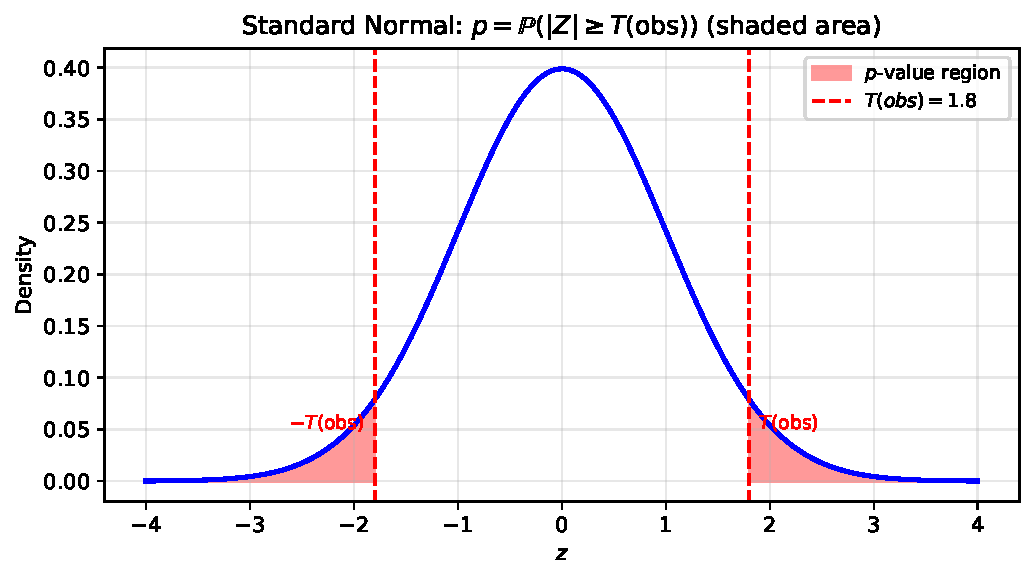
\includegraphics[width=0.48\textwidth]{normal_pvalue}
\end{center}

The figure above shows the $p$-value graphically: it is the area of the
tail of the distribution beyond the observed statistic.  A small tail area
(small $p$) means the observed value is unlikely under $\mathcal{H}_0$.

\end{frame}

%% ------------------------------------------------------------------
\begin{frame}[allowframebreaks]{2.5.2 Two Fundamental Goodness-of-Fit Tests}

We introduce the two most fundamental goodness-of-fit tests using three
concrete sets of $n = 50$ points from $[0,1)$, chosen to illustrate three
qualitatively different situations:

\begin{itemize}
  \item \textbf{Set A} (blue): generated by PCG64 via NumPy's
    \texttt{default\_rng}.  This represents a high-quality pseudorandom
    sequence and serves as the baseline.
  \item \textbf{Set B} (red): a biased nonlinear transform of Set~A,
    given by $u_i^B = (e^{u_i^A - 1} - m)/(M - m)$, where $m$ and $M$
    are the minimum and maximum of the transformed values.  This set is
    skewed heavily toward 0 and should be detected as non-uniform.
  \item \textbf{Set C} (green): a quasi-random equispaced sequence,
    $u_i = i/(n+1)$ for $i=1,\ldots,n$.  This set is ``too uniformly
    distributed'' to be random and illustrates the need for second-level
    testing (Section~2.5.6).
\end{itemize}

\begin{center}
  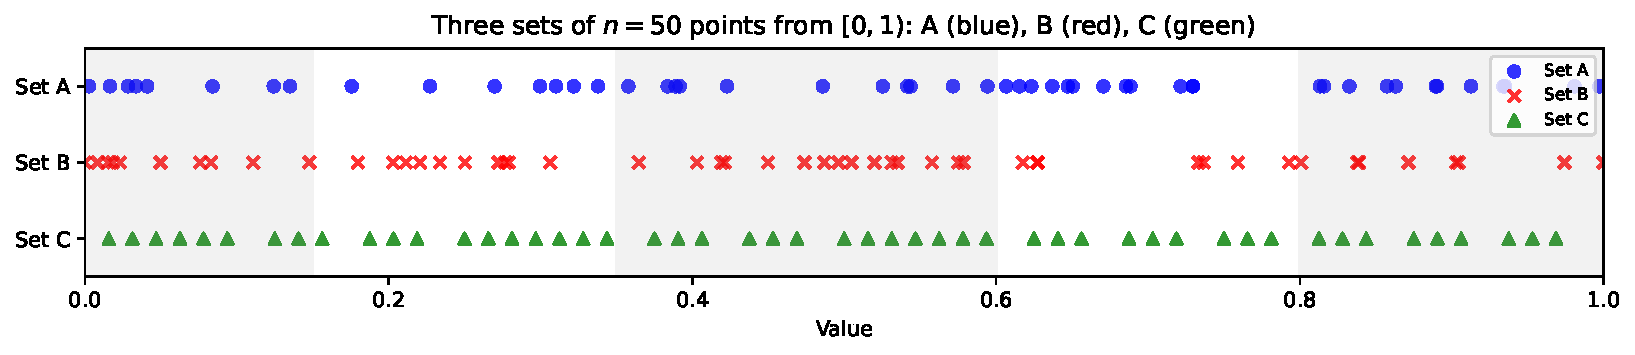
\includegraphics[width=0.82\textwidth]{sets_abc}
\end{center}

\framebreak

\begin{block}{2.5.2.1 Kolmogorov-Smirnov (KS) Goodness-of-Fit Test}
The KS test compares the \textbf{empirical cumulative distribution function}
(empirical c.d.f.) to the theoretical c.d.f.\ of $\mathcal{U}[0,1)$.

The \textbf{empirical c.d.f.} $\hat{F}_n(t)$ is the step function that
records the fraction of observed values at or below $t$:
\[
  \hat{F}_n(t) \;=\; \frac{1}{n}\sum_{i=1}^n \mathbf{1}(U_i \le t).
\]
Here $\mathbf{1}(U_i \le t)$ (the indicator function, pronounced ``1 if
$U_i \le t$, and 0 otherwise'') equals 1 when the $i$-th observation is at
most $t$, and 0 when it exceeds $t$.  So $\hat{F}_n(t)$ simply counts the
proportion of the $n$ sample values that do not exceed $t$.

For a truly uniform $\mathcal{U}[0,1)$ distribution, the theoretical c.d.f.\
is $F(t) = t$ (the diagonal line from $(0,0)$ to $(1,1)$).

The \textbf{KS statistic} $D_n$ measures the largest gap between the
empirical and theoretical c.d.f.s:
\[
  D_n \;=\; \sup_{0 \le t \le 1} \bigl|\hat{F}_n(t) - t\bigr|.
\]
Here $\sup$ (supremum, from Latin ``supremum'' meaning the least upper bound)
denotes the maximum over all values of $t \in [0,1]$.  A large $D_n$ means
the empirical distribution deviates substantially from uniform.
\end{block}

\textbf{Computing $D_n$ in practice.}
Because $\hat{F}_n(t)$ is a step function that only changes at the sample
values, the supremum is attained at one of those jumps.  Sort the sample:
$U_{(1)} \le U_{(2)} \le \cdots \le U_{(n)}$ (where $U_{(i)}$ denotes the
$i$-th smallest value, called the \emph{$i$-th order statistic}).  Then:
\[
  D_n^+ \;=\; \max_{1 \le i \le n}\!\left(\frac{i}{n} - U_{(i)}\right),\quad
  D_n^- \;=\; \max_{1 \le i \le n}\!\left(U_{(i)} - \frac{i-1}{n}\right),\quad
  D_n \;=\; \max(D_n^+,\, D_n^-).
\]
$D_n^+$ captures cases where the empirical c.d.f.\ lags behind the diagonal
(too few small values), and $D_n^-$ captures cases where it runs ahead (too
many small values).

The $p$-value with the finite-sample correction (Equation 2.5.8):
\[
  p \;=\; 1 - K\!\left(\sqrt{n}\,D_n \;+\; \frac{1}{6\sqrt{n}}
          \;+\; \frac{\sqrt{n}\,D_n - 1}{4n}\right).
\]
Here $K(\cdot)$ is the Kolmogorov distribution function, a mathematical
special function.  Critical values at common significance levels $\alpha$
(alpha, the probability of a false rejection): $\lambda_{0.10} = 1.224$,
$\lambda_{0.05} = 1.358$, $\lambda_{0.01} = 1.628$.

\framebreak

\begin{center}
  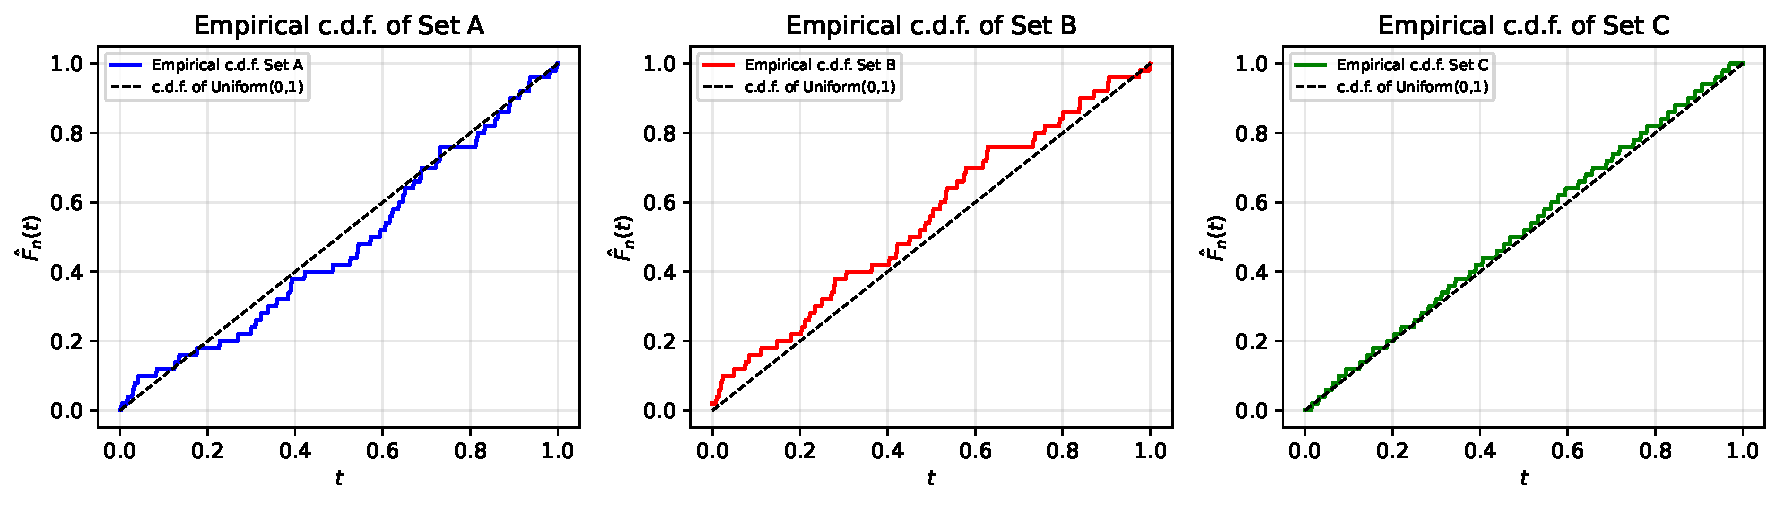
\includegraphics[width=0.85\textwidth]{ecdf_abc}
\end{center}

The figure shows the three empirical c.d.f.s overlaid on the diagonal
$F(t) = t$.  Set~A (blue) tracks the diagonal closely --- as expected for
a good pseudorandom sequence.  Set~B (red) deviates noticeably, rising
steeply near 0 because many values cluster there.  Set~C (green) matches
the diagonal so well it is nearly invisible --- which is actually
\emph{suspicious}, because genuinely random sequences never fit the
theoretical c.d.f.\ this precisely.

\begin{center}
  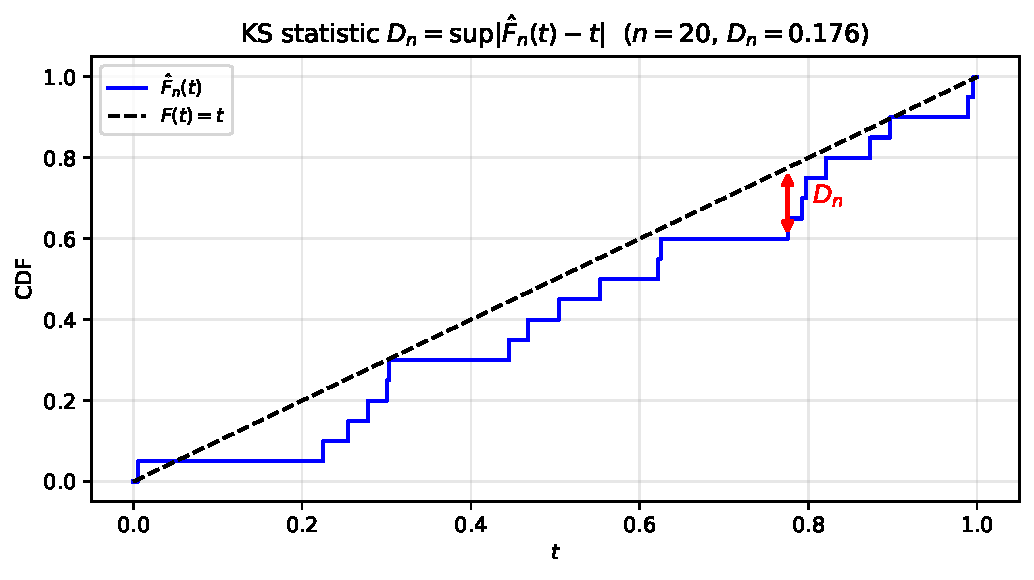
\includegraphics[width=0.52\textwidth]{ks_illustration}
\end{center}

\textbf{KS test results for Sets A, B, C} (Example~2.5.1, $n=50$):
\begin{center}
\begin{tabular}{lccc}
  \toprule
  & Set A & Set B & Set C \\
  \midrule
  $D_n$ (observed) & 0.1192 & 0.2266 & 0.0462 \\
  $p$-value & 44.17\% & 0.99\% & 99.97\% \\
  Conclusion & not rejected & \textbf{rejected} & not rejected \\
  \bottomrule
\end{tabular}
\end{center}

Set~B is correctly rejected because its $p$-value ($0.99\%$) is below the
conventional threshold of 1\%.  Set~C is not rejected at this level because
its $p$-value ($99.97\%$) is very high --- but this high value is itself a
warning sign.  Second-level testing (Section~2.5.6) is needed to detect it.

\framebreak

\begin{block}{2.5.2.2 Chi-Square ($\chi^2$) Goodness-of-Fit Test}
The chi-square (written $\chi^2$, where $\chi$ is the Greek letter chi,
pronounced ``kai'') test partitions $[0,1)$ into $k$ (k) intervals
(called \emph{bins}) with theoretical probabilities $p_1, p_2, \ldots, p_k$
(which must sum to 1) under $\mathcal{H}_0$.  We generate $r$ (r) independent
observations; let $O_i$ (O subscript i, the observed count) be the number
that fall into bin $i$, and let $E_i = r\,p_i$ (E subscript i, the
expected count) be the number expected under $\mathcal{H}_0$.

The chi-square statistic is:
\[
  X_k^2 \;=\; \sum_{i=1}^k \frac{(O_i - r\,p_i)^2}{r\,p_i}
           \;=\; \sum_{i=1}^k \frac{O_i^2}{r\,p_i} \;-\; r.
\]
Here $\Sigma$ (Sigma, uppercase, meaning ``sum over'') adds the contribution
from each bin $i = 1, 2, \ldots, k$.  Each term $(O_i - rp_i)^2 / (rp_i)$
is the squared deviation between the observed and expected count for bin $i$,
normalised (divided) by the expected count.  If all deviations are small,
$X_k^2$ is small, indicating the data fit the uniform distribution well.

As $r \to \infty$ (as the number of observations grows), $X_k^2$ converges
in distribution to $\chi^2_{k-1}$ (chi-square with $k-1$ degrees of
freedom), a standard probability distribution whose quantiles are tabulated.

\textbf{Practical rule}: each bin should have $E_i = r\,p_i \ge 5$ expected
observations to ensure the chi-square approximation is reliable.  With
uniform bins of size $1/k$, this requires $r \ge 5k$.
\end{block}

\textbf{Chi-square results for Sets A, B, C} (Example~2.5.2, $k=5$ bins,
$r=50$):
\begin{center}
\begin{tabular}{lccc}
\toprule
& Set A & Set B & Set C \\
\midrule
$X^2$ (observed) & 7.32 & 16.25 & 0.24 \\
$p$-value ($\chi^2_4$) & 11.99\% & \textbf{0.27\%} & 99.35\% \\
\bottomrule
\end{tabular}
\end{center}

Set~B is again rejected (0.27\% $<$ 1\%), while Set~C again escapes
detection at the first level (99.35\%).

\begin{center}
  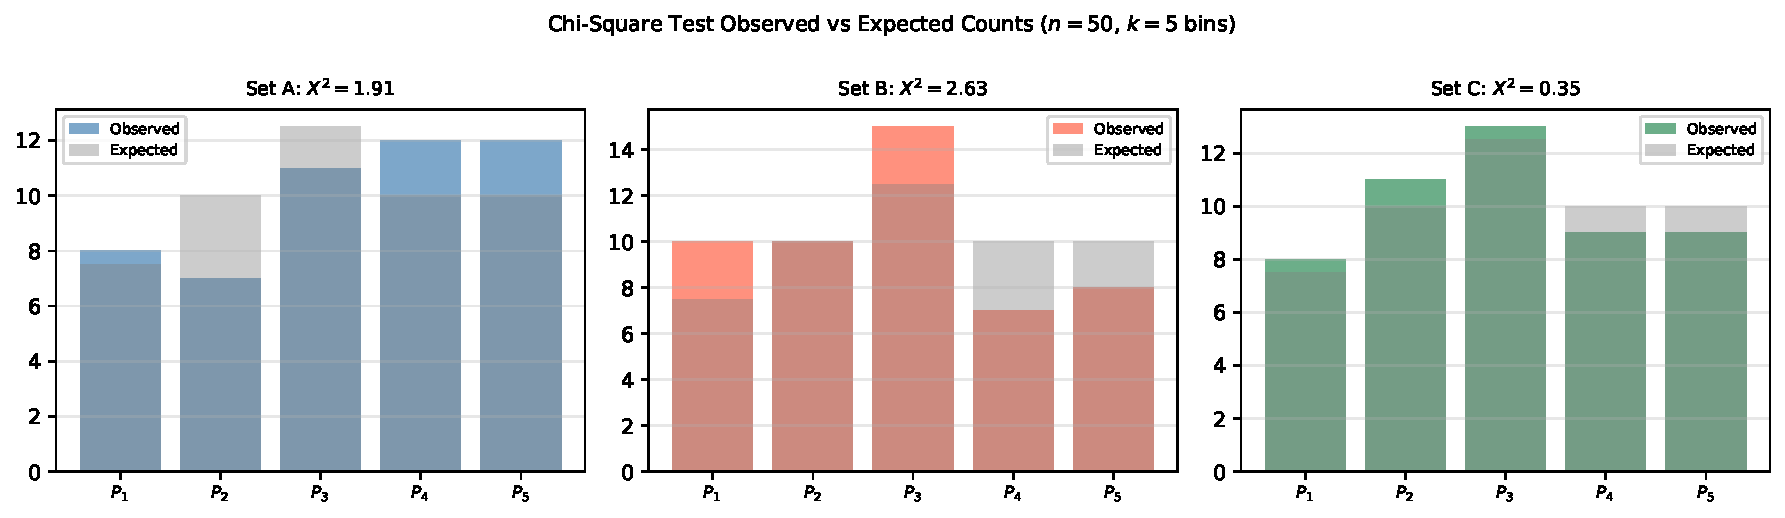
\includegraphics[width=0.82\textwidth]{chisq_hist}
\end{center}

\framebreak

\textbf{2.5.2.3 Frequency of Pairs (Serial) Test.}

A critical limitation of both the KS and chi-square tests above is that
they examine each output number \emph{individually}, one at a time.  They
cannot detect correlations \emph{between} consecutive numbers.  The
\textbf{serial test} (also called the frequency of pairs test) extends the
chi-square idea to two dimensions.

\textbf{Procedure:} group the sequence into $r = 25$ consecutive
\emph{pairs} $(u_{2i-1},\, u_{2i})$ for $i = 1, \ldots, r$, divide the
unit square $[0,1)^2$ into $L^2 = 9$ equal sub-squares (using $L = 3$
divisions per axis), count how many pairs fall into each sub-square, and
apply the chi-square test.  Under $\mathcal{H}_0$, each sub-square has
probability $1/L^2 = 1/9$, so we expect $r/9 \approx 2.78$ pairs per
sub-square.

\begin{center}
  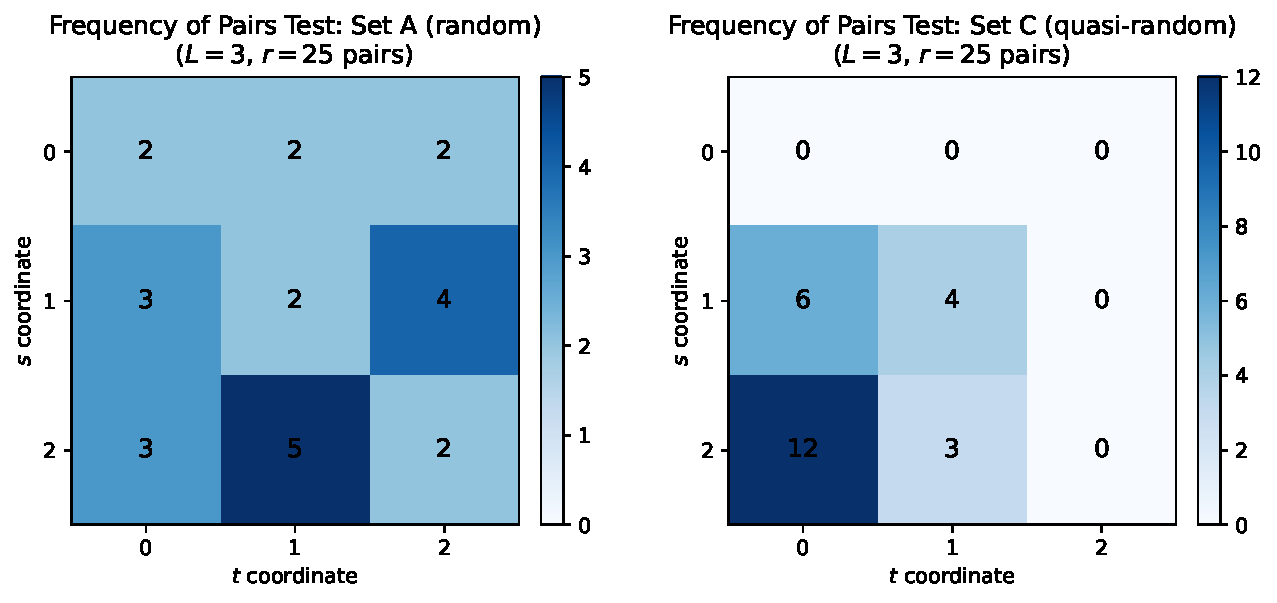
\includegraphics[width=0.82\textwidth]{freq_pairs_test}
\end{center}

The figure shows the expected and observed pair counts for each set.  For
Set~C (the quasi-random equispaced sequence), the pairs $(u_1, u_2)$,
$(u_3, u_4)$, etc.\ form a perfectly regular grid --- the $p$-value is
effectively $0\%$, conclusively detecting the sequential structure.
Importantly, when Set~C is randomly shuffled (reordering the 50 values in
random order to get Set~$C'$), the pairs test \emph{passes}: shuffling
destroys the pairwise structure while preserving the marginal distribution.
This demonstrates that quasi-randomness is a property of the \emph{ordering}
of values, not of the values themselves.

\end{frame}

%% ------------------------------------------------------------------
\begin{frame}[fragile]{2.5.2 Python Code: KS, Chi-Square, and Pairs Tests}

\begin{lstlisting}[style=python]
import numpy as np
from scipy import stats

rng = np.random.default_rng(seed=0)
n   = 50
# Set A: PCG64 pseudorandom
A = rng.random(n)
# Set B: biased nonlinear transform  (skewed toward 0)
eps = 1e-7
raw = np.exp(A - 1) - 1 - eps
B   = (raw - raw.min()) / (raw.max() - raw.min())
# Set C: quasi-random equispaced (Halton-like)
C   = np.arange(1, n + 1) / (n + 1)

# --- KS test against U[0,1) ----------------------------------------
for name, seq in [("A", A), ("B", B), ("C", C)]:
    stat, p = stats.kstest(seq, 'uniform')
    print(f"KS  Set {name}: D={stat:.4f}, p={p:.4f}")

# --- Chi-square test with 5 non-uniform bins -----------------------
bins  = [0, 0.15, 0.35, 0.60, 0.80, 1.0]
probs = [0.15, 0.20, 0.25, 0.20, 0.20]    # must sum to 1.0
for name, seq in [("A", A), ("B", B), ("C", C)]:
    obs, _ = np.histogram(seq, bins=bins)
    exp    = [n * p for p in probs]
    chi2, p_val = stats.chisquare(obs, exp)
    print(f"Chi2 Set {name}: X2={chi2:.3f}, p={p_val:.4f}")

# --- Frequency of Pairs (Serial) test: L=3, r=25 pairs -----------
for name, seq in [("A", A), ("B", B), ("C", C)]:
    L    = 3
    # Take first 50 values as 25 consecutive pairs
    pairs   = np.column_stack([seq[::2][:25], seq[1::2][:25]])
    # Assign each pair to one of the 9 sub-squares
    indices = np.floor(L * pairs).astype(int).clip(0, L - 1)
    keys    = indices[:, 0] * L + indices[:, 1]  # 0..8
    obs     = np.bincount(keys, minlength=L * L)
    exp     = [len(pairs) / (L * L)] * (L * L)
    chi2, p_val = stats.chisquare(obs, exp)
    print(f"Pairs Set {name}: X2={chi2:.3f}, p={p_val:.4f}")
\end{lstlisting}

\end{frame}

%% ------------------------------------------------------------------
\begin{frame}[allowframebreaks]{2.5.3 Tests Based on Balls-and-Boxes Schemes}

Many classical PRNG tests can be unified within the elegant
\textbf{balls-and-boxes framework}.  The general setup is this: imagine
placing $r$ (r) balls into $k$ (k) boxes independently and uniformly at
random, so each ball independently chooses a box uniformly from $\{1, \ldots, k\}$.
Under the null hypothesis $\mathcal{H}_0$ (that the sequence is truly random),
the occupancy counts follow a \emph{multinomial distribution}.

To convert a PRNG output sequence into this framework: form $r$ vectors
$\mathbf{u}_1, \ldots, \mathbf{u}_r$ each of dimension $m$ (m), partition
$[0,1)^m$ into $k = L^m$ equal sub-hypercubes (where $L$ is the number of
divisions per axis), and map each vector $\mathbf{u}_i$ to the sub-hypercube
it falls into (the ``box'').  The choice of $m$, $L$, and $k$ defines the
specific test.

\begin{center}
  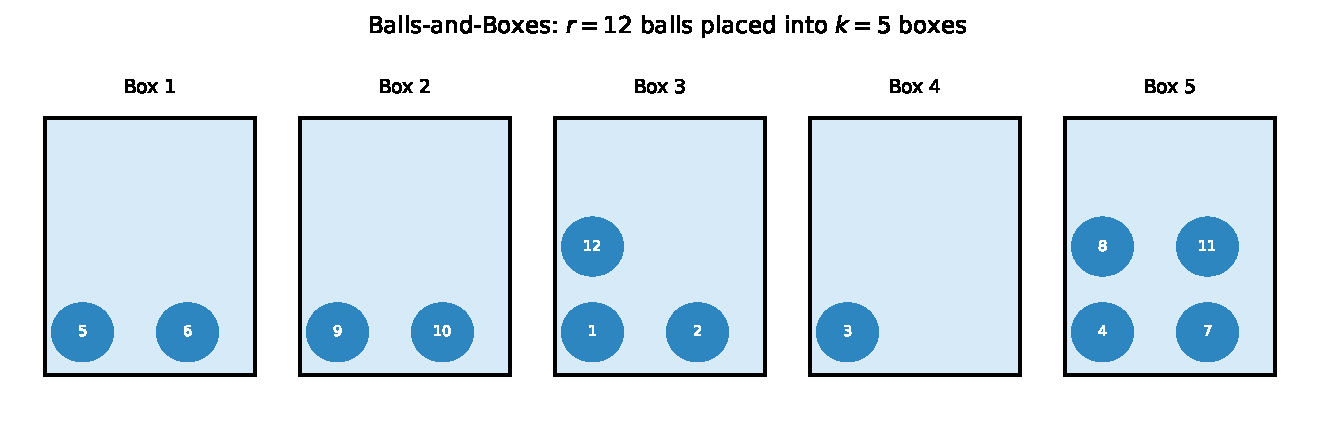
\includegraphics[width=0.62\textwidth]{balls_boxes}
\end{center}

\framebreak

\textbf{The Birthday Problem.}
The classical birthday problem asks: how many students must be in a room
before there is a better-than-even chance that at least two share a birthday?
Assuming birthdays are uniformly distributed among $k = 365$ days, the
probability that all $r$ students have \emph{distinct} birthdays is:
\[
  \frac{(365)_r}{365^r}
  \;=\; \prod_{j=1}^{r-1}\!\left(1-\frac{j}{365}\right).
\]
Here $(365)_r = 365 \times 364 \times \cdots \times (365-r+1)$ is the
\textbf{falling factorial} (the product of $r$ integers counting down from
365), and $\prod$ (Pi, uppercase, meaning ``product over'') multiplies the
$r-1$ terms together.  The probability of at least one collision is
$1 - (365)_r / 365^r$.

\begin{exampleblock}{Worked Computation: Birthday Probability}
With $r = 23$ students and $k = 365$ days:
\[
  p = 1 - \frac{365 \times 364 \times \cdots \times 343}{365^{23}}
  \approx 1 - e^{-23 \times 22 / (2 \times 365)}
  = 1 - e^{-\lambda},\quad \lambda = \frac{23^2}{2 \times 365} \approx 0.725.
\]
Here $e \approx 2.718$ is Euler's number (the base of the natural logarithm).
So $p \approx 1 - e^{-0.725} \approx 0.516$: with 23 students, there is
already a 51.6\% chance of a shared birthday.  With $r = 70$ students,
$\lambda \approx 6.7$ and $p \approx 1 - e^{-6.7} \approx 0.999$.
\end{exampleblock}

For general $k$ boxes and $r$ balls, the Poisson approximation to the
collision probability is:
\[
  p_{k,r} \;\approx\; 1 - \exp\!\left(-\frac{r^2}{2k}\right). \tag{2.5.12}
\]
Here $\exp(\cdot)$ denotes the exponential function ($e$ raised to a power),
and $r^2/(2k)$ is the expected number of collisions (denoted $\lambda$,
lambda).

\begin{center}
  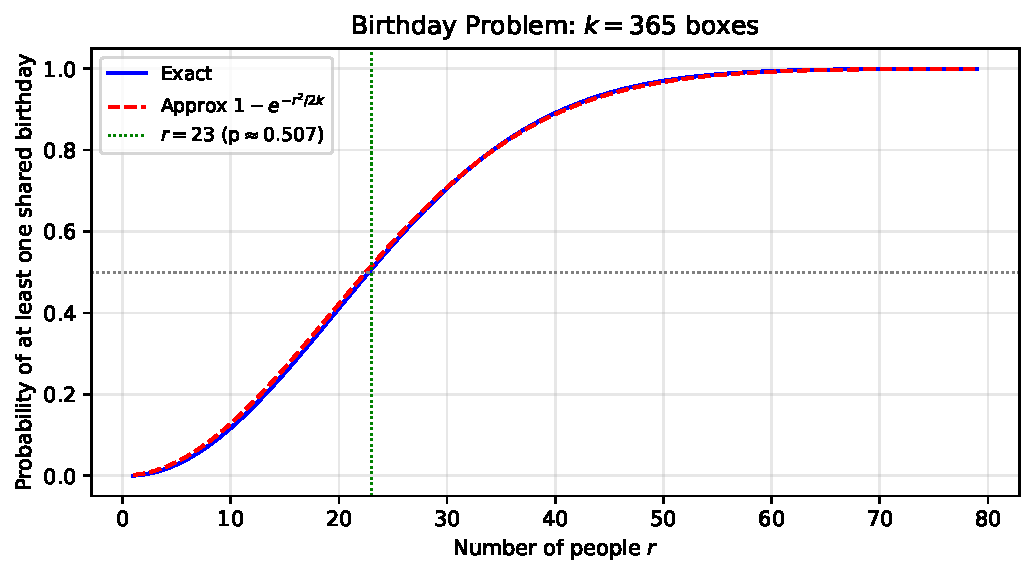
\includegraphics[width=0.52\textwidth]{birthday_problem}
\end{center}

\framebreak

\begin{block}{Collision Test}
A \emph{collision} occurs when a ball lands in a box that already contains
at least one ball.  Let $C_{k,r}$ (C subscript k,r) be the total number of
collisions after placing $r$ balls in $k$ boxes.  The exact probability of
exactly $c$ (c) collisions is:
\[
  \mathbb{P}(C_{k,r} = c)
  \;=\; \frac{k(k-1)\cdots(k-r+c+1)\;\cdot\;S_2(r,\,r-c)}{k^r}, \tag{2.5.13}
\]
where $S_2(r, s)$ (S sub 2, of r and s) is the \textbf{Stirling number of
the second kind}: the number of ways to partition a set of $r$ labeled
objects into exactly $s$ non-empty, unlabeled subsets.

The \textbf{Poisson approximation}: when $r$ and $k$ grow large together
with $r^2 / (2k) \to \lambda$ (lambda, a fixed positive constant):
\[
  \mathbb{P}(C_{k,r} = c) \;\to\; \frac{\lambda^c}{c!}\,e^{-\lambda}. \tag{2.5.14}
\]
Here $c!$ (c factorial) is $1 \times 2 \times \cdots \times c$.  This says
that $C_{k,r}$ follows approximately a Poisson distribution with mean
$\lambda = r^2 / (2k)$.
\end{block}

\begin{block}{Expected Number of Collisions}
The expected (average) number of collisions is:
\[
  \mathbb{E}C_{k,r}
  \;=\; r \;-\; k\left(1 - \left(1-\frac{1}{k}\right)^r\right)
  \;\approx\; \frac{r^2}{2k}.
\]
Here $\mathbb{E}$ (E with a double-struck style, read ``expected value of'')
denotes the average of $C_{k,r}$ over all possible random outcomes.  The
factor $(1 - 1/k)^r$ is the probability that a given box remains empty
after all $r$ balls are thrown.

\textbf{Worked example:} with $r = 2^{14} = 16{,}384$ balls and
$k = 2^{20} \approx 1{,}048{,}576$ boxes:
\[
  \mathbb{E}C_{k,r} \;\approx\; \frac{(2^{14})^2}{2 \cdot 2^{20}}
  = \frac{2^{28}}{2^{21}} = 2^7 = 128.
\]
We expect about 128 collisions.  A PRNG producing significantly more or fewer
collisions than this expected value fails the collision test.
\end{block}

\begin{center}
  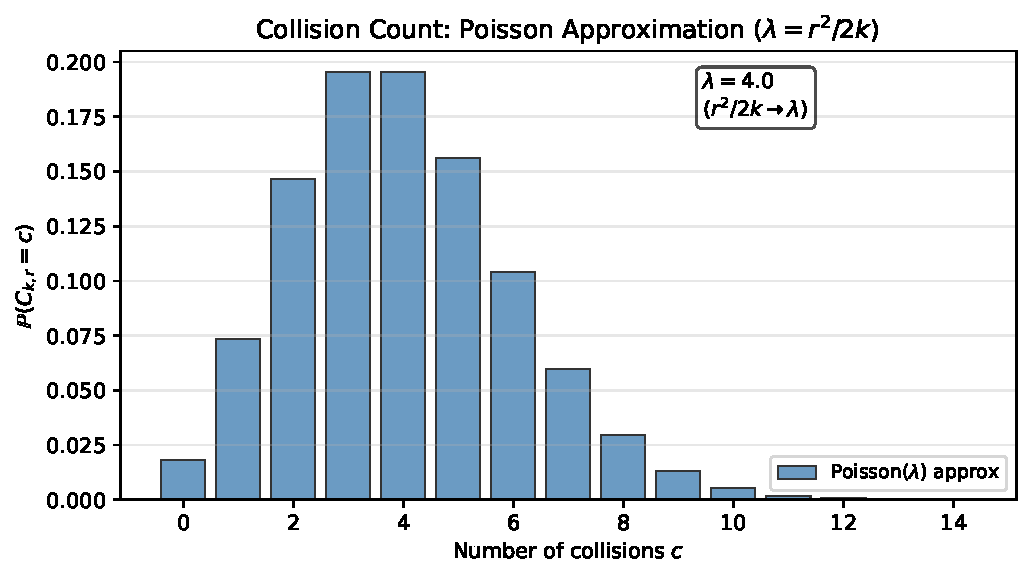
\includegraphics[width=0.52\textwidth]{collision_distribution}
\end{center}

\framebreak

\textbf{Birthday Spacing Test (Marsaglia).}
This is one of the most stringent tests for LCGs.  Given a long sequence
of $R \times n$ bits (where $R$ is the number of repetitions and
$n = m \times r$ with $m = 25$ and $r = 2^9 = 512$), the test proceeds
as follows:
\begin{enumerate}
  \item Split the sequence into $R$ non-overlapping blocks, each of length $n$.
  \item In each block, form $r = 512$ values of $m = 25$ bits each
    (interpreting each 25-bit string as an integer in $\{0, \ldots, 2^{25}-1\}$).
    These are the ``birthdays'', with ``year length'' $k = 2^{25}$.
  \item Sort the birthdays and compute the $r-1$ consecutive spacings (gaps
    between adjacent sorted values).
  \item Count $K$, the number of \emph{equal spacings} (spacings that appear
    more than once).  Under $\mathcal{H}_0$, $K$ approximately follows a
    Poisson distribution with mean $\lambda = r^3 / (4k)$.
  \item Apply a chi-square test to the $R$ values of $K$ across all blocks.
\end{enumerate}
This test fails the MATLAB \texttt{rand('state')} LCG with a $p$-value of
$4.12 \times 10^{-100}$ --- a number so astronomically small that the
generator is conclusively non-random.

\medskip
\textbf{Poker Test.}
Group $n = 5r$ integers $y_1, \ldots, y_n \in \{0, \ldots, M-1\}$ into
$r$ groups of 5.  For each group, count the number of \emph{distinct values}
$s$ among the five (analogous to counting distinct card denominations in a
poker hand).  The theoretical probability of a 5-tuple having exactly $s$
distinct values is:
\[
  p_s \;=\; \frac{M(M-1)\cdots(M-s+1)\;\cdot\;S_2(5,\,s)}{M^5},
\]
where the Stirling numbers for $s = 1, \ldots, 5$ are
$S_2(5,1) = 1$,\ $S_2(5,2) = 15$,\ $S_2(5,3) = 25$,\ $S_2(5,4) = 10$,\
$S_2(5,5) = 1$.  A chi-square test with $k-1 = 4$ degrees of freedom is
then applied to the observed frequencies.

\begin{alertblock}{Key Insight: Balls-and-Boxes Unifies Many Classical Tests}
The balls-and-boxes framework shows that the birthday, collision, spacing,
and poker tests are all instances of the same combinatorial idea.  The
birthday spacing test is especially sensitive to LCGs because the lattice
structure causes the spacings between sorted values to be non-uniform ---
certain spacing values are far more common than they should be, and this
regularity is detected by counting equal spacings.
\end{alertblock}

\end{frame}

%% ------------------------------------------------------------------
\begin{frame}[allowframebreaks]{2.5.4 Tests Based on Random Walks}

Random walk tests take a different approach: they convert a binary sequence
into a one-dimensional random walk and then exploit the rich mathematical
theory of random walks to construct tests with precisely known distributions
under $\mathcal{H}_0$.

A \textbf{random walk} (also called a drunkard's walk) is a sequence of
positions on the number line where each step is equally likely to be $+1$
(one step right) or $-1$ (one step left).  If the bits are truly random,
the walk is \emph{symmetric}: it has no tendency to drift in either
direction.  Departures from symmetry indicate biased bit generation.

\begin{block}{From Bits to a Random Walk}
Given bits $b_1, b_2, \ldots \in \{0,1\}$, define the centred increments
and partial sums:
\[
  X_i \;=\; 2B_i - 1 \;\in\; \{-1,\,+1\},\quad
  S_0 \;=\; 0,\quad
  S_k \;=\; \sum_{i=1}^k X_i.
\]
Here $X_i$ (X subscript i) is $+1$ when bit $b_i = 1$ (step right) and
$-1$ when $b_i = 0$ (step left).  The running sum $S_k$ (S subscript k)
gives the position of the walk after $k$ steps.  Under $\mathcal{H}_0$,
$\mathbb{E}[X_i] = 0$ (the expected step is zero, so there is no drift)
and $\mathrm{Var}(X_i) = 1$ (the variance of each step is 1).
\end{block}

\begin{center}
  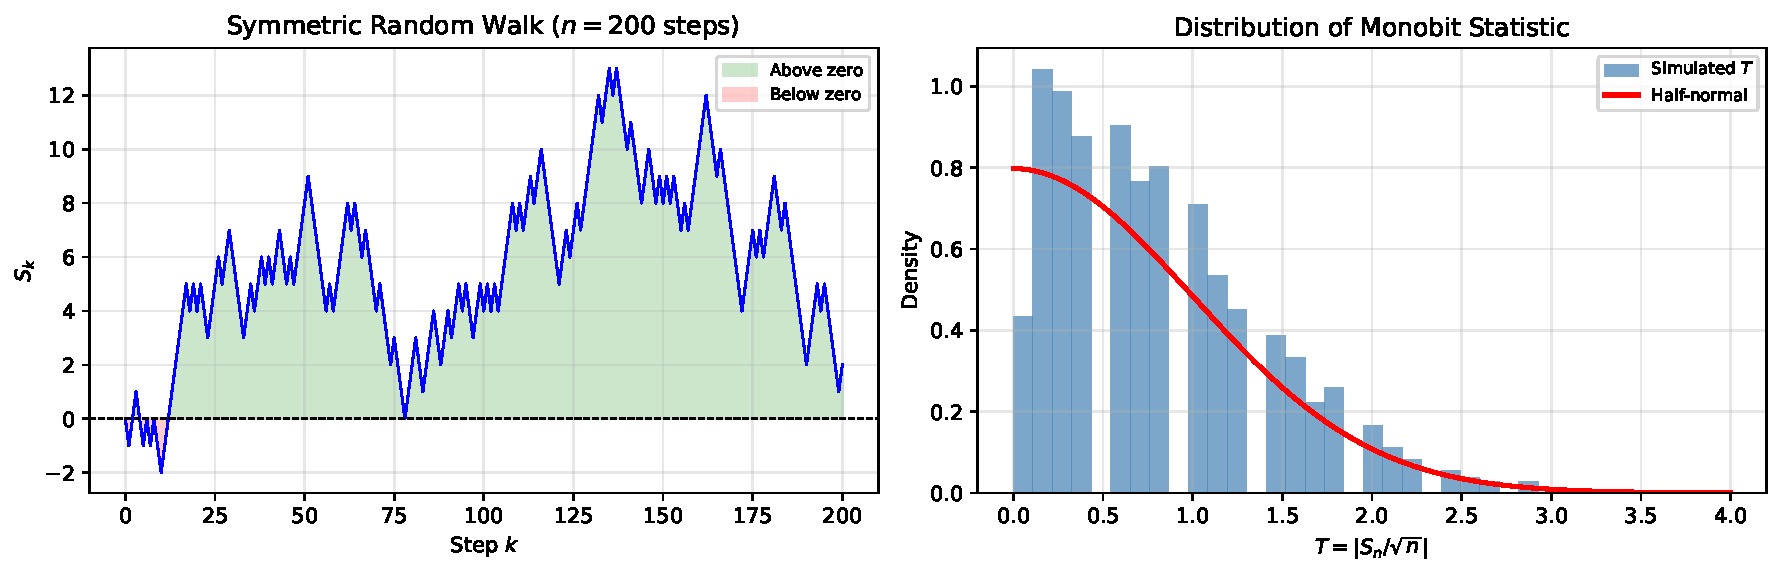
\includegraphics[width=0.76\textwidth]{random_walk}
\end{center}

The figure shows a typical symmetric random walk of length $n = 1000$.
The walk oscillates without systematic drift.  Notice that despite having
no systematic bias, the walk can stray far from 0 for extended periods ---
this is a well-known property of random walks.

\framebreak

\begin{block}{Frequency (Monobit) Test}
The simplest random walk test asks: is the final position $S_n$ consistent
with a zero-mean symmetric walk?  By the Central Limit Theorem (CLT ---
the theorem stating that the sum of many independent random variables is
approximately normally distributed), $S_n / \sqrt{n}$ converges in
distribution to $\mathcal{N}(0,1)$ (the standard normal distribution,
a bell curve centred at 0 with standard deviation 1) as $n \to \infty$.

The test statistic is $T_{\mathrm{obs}} = |S_n| / \sqrt{n}$ (the absolute
value of the normalised walk position), and the $p$-value is:
\[
  p \;=\; \mathrm{erfc}\!\left(\frac{T_{\mathrm{obs}}}{\sqrt{2}}\right).
\]
Here $\mathrm{erfc}(x)$ (complementary error function, pronounced
``erfc of x'') is defined as
$\mathrm{erfc}(x) = (2/\sqrt{\pi})\int_x^\infty e^{-t^2}\,dt$, where
$\pi$ (pi) $\approx 3.14159$.  This gives the probability that a standard
normal variable has absolute value at least $T_{\mathrm{obs}}$.

The monobit test checks whether the number of 0-bits and 1-bits is
approximately equal.  If the PRNG produces more 1s than 0s (or vice versa),
$|S_n|$ will be large, giving a small $p$-value and rejecting $\mathcal{H}_0$.
\end{block}

\begin{block}{Frequency Test in Blocks}
The global monobit test can miss a generator that is balanced overall but
has local imbalances.  The block frequency test detects these:

Split $n = m \times r$ bits (m bits per block, r blocks total) into $r$
blocks of length $m$.  For block $i$, let $S_m^{(i)}$ be the walk position
at the end of that block (the sum of $\pm 1$ values within block $i$).
Define the normalised end positions $Z_i = S_m^{(i)} / \sqrt{m}$.  For
large $m$, these are approximately i.i.d.\ $\mathcal{N}(0,1)$.

The test statistic:
\[
  T_{\mathrm{obs}} \;=\; \frac{1}{m}\sum_{i=1}^r \bigl(S_m^{(i)}\bigr)^2
  \;\approx\; \chi^2_r \quad (\text{chi-square with }r\text{ degrees of freedom}).
\]
A generator with a long-range trend in bit frequencies (e.g., more 1s in
the first half of the sequence and more 0s in the second half) would pass
the monobit test but fail the block frequency test, because the individual
block sums $S_m^{(i)}$ would not all be near zero.
\end{block}

\framebreak

\begin{block}{Arcsine Law Based Test}
A remarkable and counterintuitive property of the symmetric random walk is
the \textbf{Arcsine Law} (Feller, 1968).  Define $L_{2r}^+$ as the total
number of time steps at which the walk is in positive territory (i.e., the
number of indices $k \in \{1, \ldots, 2r\}$ with $S_k > 0$).  Intuitively,
one might expect the walk to spend about half its time above zero and half
below.  In fact, the opposite is true: the walk is most likely to spend
\emph{almost all} its time on one side:
\[
  \lim_{r\to\infty}
  \mathbb{P}\!\left(\frac{L_{2r}^+}{2r} \;\le\; w\right)
  \;=\; \frac{2}{\pi}\arcsin\!\sqrt{w}, \quad w \;\in\; [0,1].
\]
Here $\arcsin$ (arcsine, the inverse of the sine function) and $\pi$ (pi)
$\approx 3.14159$ appear in the formula.  The density
$\frac{d}{dw}\!\left[\frac{2}{\pi}\arcsin\!\sqrt{w}\right]
= \frac{1}{\pi\sqrt{w(1-w)}}$ is U-shaped: it is largest near $w=0$ and
$w=1$.  Spending exactly half the time above zero (the ``intuitive'' outcome)
actually has probability \emph{zero} under this distribution.

This result forms the basis of a test: compute $T_{\mathrm{obs}}
= L_{2r}^+ / (2r)$ from the PRNG output and check whether it follows the
arcsine distribution.  The $p$-value is:
$p \approx 1 - \frac{2}{\pi}\arcsin\!\sqrt{T_{\mathrm{obs}}}$.
\end{block}

\begin{center}
  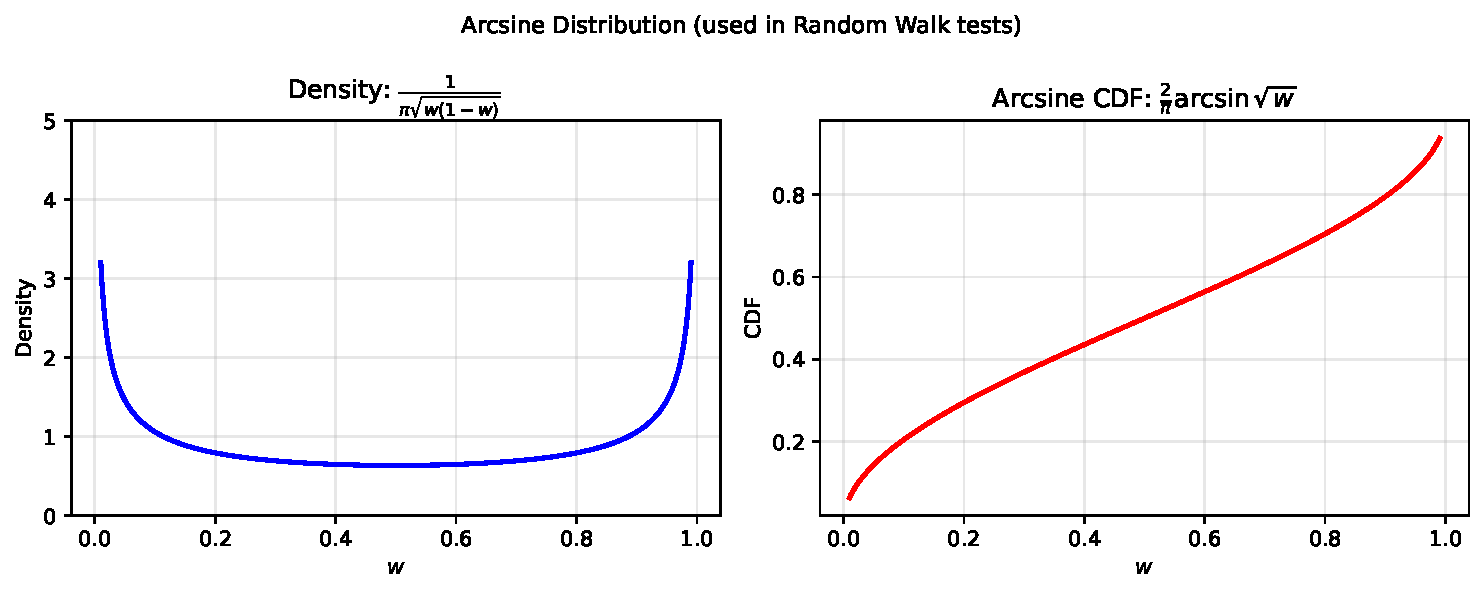
\includegraphics[width=0.52\textwidth]{arcsine_law}
\end{center}

\framebreak

\begin{block}{Random Excursion Test (NIST)}
An \emph{excursion} is a segment of the walk between two consecutive
returns to zero: it starts and ends at $S_k = 0$ (position zero) and
does not touch zero in between.  Let $J_n$ denote the number of complete
returns to zero ($S_k = 0$ for $k = 1, \ldots, n$).

Under $\mathcal{H}_0$, the distribution of $J_n$ is known: the NIST
standard recommends rejecting $\mathcal{H}_0$ if
$J_n < 0.008\sqrt{n}$ (too few returns to zero, meaning the walk is
drifting rather than oscillating).

For each excursion, let $L(x)$ (L of x) count the number of visits to
state $x \in \{1, 2, \ldots, 7\}$ (seven specific positive states of
interest).  The theoretical distribution of $L(x)$ under $\mathcal{H}_0$
is:
\[
  \mathbb{P}(L(x) = k) \;=\;
  \begin{cases}
    1 - \dfrac{1}{2|x|}, & k = 0, \\[8pt]
    \dfrac{1}{4x^2}\!\left(1-\dfrac{1}{2|x|}\right)^{k-1}, & k \;\ge\; 1.
  \end{cases} \tag{2.5.22}
\]
Here $|x|$ (absolute value of $x$) equals $x$ since we consider only
positive states.  For each state $x$, count observed visit frequencies
$E_k(x)$ for $k = 0, 1, 2, 3, 4$ (merging all $k \ge 5$ into one
category), across all excursions, and apply a chi-square test with 5
degrees of freedom.  If the PRNG output is truly random, the visits
to each state follow this geometric-like distribution.
\end{block}

\begin{alertblock}{Key Insight: Random Walk Tests Exploit Deep Theory}
What makes random walk tests powerful is that the distributions of
$S_n/\sqrt{n}$, $L_{2r}^+/(2r)$, and $J_n$ are known \emph{exactly}
(or with precise asymptotic corrections) from the mathematical theory
of random walks.  This allows precise $p$-value computation, unlike
some ad-hoc tests where the null distribution must be approximated
by simulation.
\end{alertblock}

\end{frame}

%% ------------------------------------------------------------------
\begin{frame}[allowframebreaks]{2.5.5 Permutation Tests}

Permutation tests take a complementary approach to random walk tests.
Instead of converting bits into walks, they convert blocks of pseudorandom
numbers into permutations and then exploit the rich combinatorial theory of
permutations to build precise statistical tests.

The key idea is that if we take $m$ (m) uniform numbers $u_1, \ldots, u_m$
and sort them to get the ranking (i.e., which is smallest, which is
second-smallest, etc.), the ranking should be uniformly distributed over
all $m!$ (m factorial) possible orderings.  Any deviation from this
uniformity reveals structure in the PRNG output.

\begin{block}{Derangements (Lemma 2.5.10)}
A \textbf{derangement} of the set $\{1, 2, \ldots, m\}$ is a permutation
$\sigma$ (sigma, lowercase) with \emph{no fixed points}: $\sigma(i) \ne i$
for all $i = 1, \ldots, m$.  In other words, not a single element stays in
its original position after the permutation.  A classic example: a
derangement of $\{1,2,3\}$ is $(2,3,1)$ --- element 1 moved to position 3,
element 2 moved to position 1, element 3 moved to position 2.

The total number of derangements of $m$ elements is:
\[
  d_m \;=\; m!\sum_{k=0}^m \frac{(-1)^k}{k!}
       \;=\; m!\!\left(1 - 1 + \frac{1}{2!} - \frac{1}{3!}
             + \cdots + \frac{(-1)^m}{m!}\right).
\]
Here $(-1)^k$ (negative one to the power k) alternates between $+1$
(when $k$ is even) and $-1$ (when $k$ is odd).  As $m \to \infty$
(as $m$ grows without bound), the fraction $d_m / m!$ converges to
$e^{-1} \approx 0.3679$ (where $e \approx 2.718$ is Euler's number).
This means approximately $36.79\%$ of all random permutations of large
sets are derangements.
\end{block}

\begin{exampleblock}{Worked Example: $m = 4$}
$d_4 = 4!\!\left(1 - 1 + \frac{1}{2} - \frac{1}{6} + \frac{1}{24}\right)
     = 24 \times \frac{3}{8} = 9$.

There are 9 derangements of $\{1, 2, 3, 4\}$ out of $4! = 24$ total
permutations.  The probability of a derangement is
$9/24 = 0.375 \approx e^{-1} = 0.3679$ (the approximation improves
with larger $m$).

One such derangement: $(2, 1, 4, 3)$ --- element 1 goes to position 2,
element 2 to position 1, element 3 to position 4, element 4 to position 3.
None of the four elements stays in its original position.
\end{exampleblock}

\framebreak

\begin{block}{Derangement Permutation Test}
The test uses $n = m \times r$ pseudorandom outputs $u_1, \ldots, u_n$,
divided into $r$ blocks of $m$ values each.
\begin{enumerate}
  \item Initialise counter $\xi = 0$ (xi, the Greek letter xi, pronounced
    ``ks-eye'' or ``zai'').
  \item For each block $i = 1, \ldots, r$: use the Fisher-Yates algorithm
    to generate a permutation $\sigma_i$ of $\{0, \ldots, m-1\}$ from
    the $m$ uniform inputs $(u_{(i-1)m+1}, \ldots, u_{im})$.  Increment
    $\xi$ if $\sigma_i$ is a derangement.
  \item Under $\mathcal{H}_0$, the expected number of derangements among
    $r$ permutations is $r e^{-1}$.  The test statistic is:
    \[
      T_{\mathrm{obs}}
      \;=\; \frac{|\xi - r\,e^{-1}|}{\sqrt{r\,e^{-1}(1 - e^{-1})}},
      \quad p = \mathrm{erfc}\!\left(\frac{T_{\mathrm{obs}}}{\sqrt{2}}\right).
    \]
\end{enumerate}

\textbf{Notation:}
$\xi$ (xi): the observed count of derangements.
$r\,e^{-1}$: the expected count of derangements (r times $1/e \approx 0.368$).
$\sqrt{r\,e^{-1}(1-e^{-1})}$: the standard deviation of the count under
$\mathcal{H}_0$ (derived from the binomial distribution with $r$ trials and
success probability $e^{-1}$).  The denominator normalises the deviation so
that $T_{\mathrm{obs}}$ follows an approximately standard normal distribution.
\end{block}

\begin{block}{Fixed-Point Permutation Test}
For each $m$-tuple, generate permutation $\sigma$ via Fisher-Yates and count
the number of fixed points: $\xi = \#\{j : \sigma(j) = j\}$ (the number
of elements that land in their original position).

Under $\mathcal{H}_0$, as $m \to \infty$, the number of fixed points $\xi$
converges in distribution to a Poisson(1) random variable (a Poisson
distribution with mean 1).  In a Poisson(1) distribution:
$\mathbb{P}(\xi = k) = e^{-1}/k!$ for $k = 0, 1, 2, \ldots$

\textbf{Test procedure:} group the $r$ observed fixed-point counts into
11 categories: $A_j = \{j\}$ for $j = 0, 1, \ldots, 9$ and
$A_{10} = \{10, 11, 12, \ldots\}$ (all values $\ge 10$).  The expected
probabilities are $p_j = e^{-1}/j!$ for $j \le 9$ and
$p_{10} = 1 - \sum_{j=0}^9 p_j$.  Apply a chi-square test with 10 degrees
of freedom.

A PRNG that produces too many or too few fixed points (compared to the
Poisson(1) prediction) fails this test.  A generator whose permutations
are not uniformly distributed will typically have the wrong fixed-point
distribution.
\end{block}

\end{frame}

%% ------------------------------------------------------------------
\begin{frame}[fragile]{2.5.5 Python Code: Permutation Tests}

\begin{lstlisting}[style=python]
import numpy as np
from scipy import stats
from math import factorial, exp

def fisher_yates(m, u):
    """Generate a permutation of {0,...,m-1} from m uniform inputs."""
    S = list(range(m))
    for i in range(m, 0, -1):
        k = int(i * u[i - 1])            # uniform index in {0,...,i-1}
        S[k], S[i - 1] = S[i - 1], S[k]  # swap
    return S

def is_derangement(sigma):
    """Return True if sigma has no fixed points."""
    return all(sigma[i] != i for i in range(len(sigma)))

rng   = np.random.default_rng(42)
m, r  = 10, 2000      # 10-tuples; 2000 repetitions
u     = rng.random(m * r)

# ---- Derangement test ------------------------------------------------
xi    = sum(is_derangement(fisher_yates(m, u[i*m:(i+1)*m]))
            for i in range(r))
e_inv = exp(-1)
T_obs = abs(xi - r * e_inv) / (r * e_inv * (1 - e_inv))**0.5
p_val = stats.erfc(T_obs / 2**0.5)
print(f"Derangements: {xi}/{r}  (expected {r*e_inv:.1f})")
print(f"  T={T_obs:.3f}  p={p_val:.4f}")

# ---- Fixed-point test ------------------------------------------------
fp_counts = []
for i in range(r):
    sigma = fisher_yates(m, u[i*m:(i+1)*m])
    fp_counts.append(sum(1 for j in range(m) if sigma[j] == j))

# Group into 11 categories (0,1,...,9, >=10)
obs    = np.bincount(np.clip(fp_counts, 0, 10), minlength=11)
probs  = np.array([exp(-1) / factorial(j) for j in range(10)])
probs  = np.append(probs, 1.0 - probs.sum())
chi2, p = stats.chisquare(obs, r * probs)
print(f"Fixed-point test: chi2={chi2:.3f}  p={p:.4f}")
\end{lstlisting}

\end{frame}

%% ------------------------------------------------------------------
\begin{frame}[allowframebreaks]{2.5.6 $p$-Values and Second-Level Testing}

A single statistical test applied to a single sequence is often not
conclusive.  A genuinely good PRNG might occasionally produce a small
$p$-value purely by chance (called a \emph{Type I error} or ``false
positive''): if we apply 100 tests at the 1\% significance level, we
expect about 1 false rejection even for a perfect generator.  Conversely,
a defective generator might happen to pass a particular test for a
particular choice of parameters.

\textbf{Second-level testing} addresses both problems by applying the same
test to \emph{many} independent sequences and checking that the collection
of resulting $p$-values is itself uniformly distributed over $[0,1)$.

\begin{block}{Why $p$-Values Are Uniform Under $\mathcal{H}_0$}
Suppose the test statistic $T$ has a continuous, strictly increasing
cumulative distribution function $F$ under $\mathcal{H}_0$.  The $p$-value
is $p = 1 - F(T)$.  Then:
\[
  \mathbb{P}(p \;\le\; t)
  \;=\; \mathbb{P}(1 - F(T) \;\le\; t)
  \;=\; \mathbb{P}(F(T) \;\ge\; 1-t)
  \;=\; \mathbb{P}(T \;\ge\; F^{-1}(1-t))
  \;=\; 1 - F(F^{-1}(1-t)) = t.
\]
So $p \sim \mathcal{U}[0,1)$ under $\mathcal{H}_0$.  This derivation uses
only the fact that $F$ is continuous and strictly increasing, so $F^{-1}$
(F inverse) is well-defined.  The conclusion: if the null hypothesis is
true, $p$-values are uniformly distributed.  Any systematic departure from
uniformity in a large collection of $p$-values is evidence of non-randomness.
\end{block}

\framebreak

\begin{block}{Second-Level Testing Procedure}
\begin{enumerate}
  \item Split a long sequence of total length $R \times n$ into $R$
    non-overlapping subsequences, each of length $n$.
  \item For subsequence $i$ ($i = 1, \ldots, R$): compute the test statistic
    $T^{(i)}$ and first-level $p$-value
    $p^{(i)} = 1 - F(T^{(i)})$.
  \item Test whether $p^{(1)}, p^{(2)}, \ldots, p^{(R)}$ are themselves
    uniformly distributed on $[0,1)$ by:
    \begin{enumerate}[(a)]
      \item Partitioning $[0,1)$ into $s$ equal bins
        $[(j-1)/s,\, j/s)$ for $j = 1, \ldots, s$.
      \item Counting $O_j = |\{i : p^{(i)} \in \text{bin } j\}|$
        (the number of first-level $p$-values falling in bin $j$).
      \item The expected count in each bin is $E_j = R/s$.
      \item Computing the chi-square statistic:
        \[
          X^2_{\mathrm{final}}
          \;=\; \sum_{j=1}^s \frac{(O_j - R/s)^2}{R/s}
          \;\approx\; \chi^2_{s-1}.
        \]
    \end{enumerate}
  \item The final $p$-value is
    $p_{\mathrm{final}} = 1 - F_{\chi^2_{s-1}}(X^2_{\mathrm{final}})$,
    where $F_{\chi^2_{s-1}}$ is the c.d.f.\ of the chi-square distribution
    with $s-1$ degrees of freedom.
\end{enumerate}
\end{block}

\begin{center}
  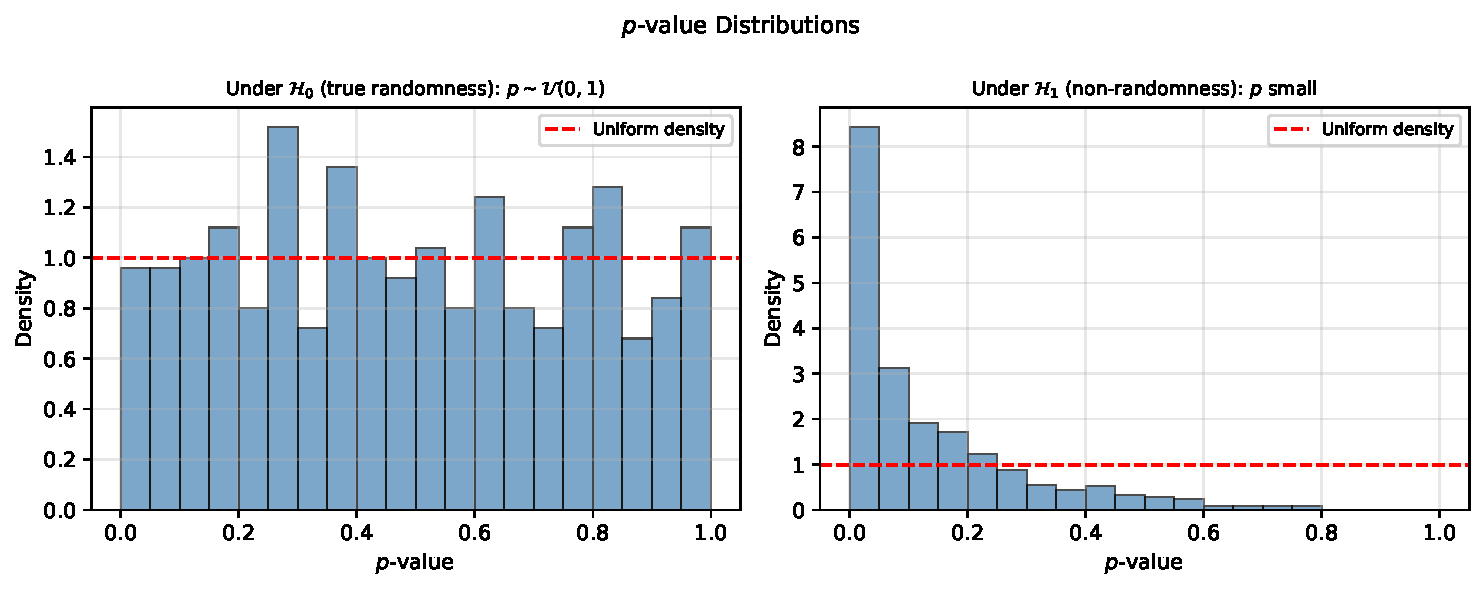
\includegraphics[width=0.76\textwidth]{pvalue_distribution}
\end{center}

\begin{center}
  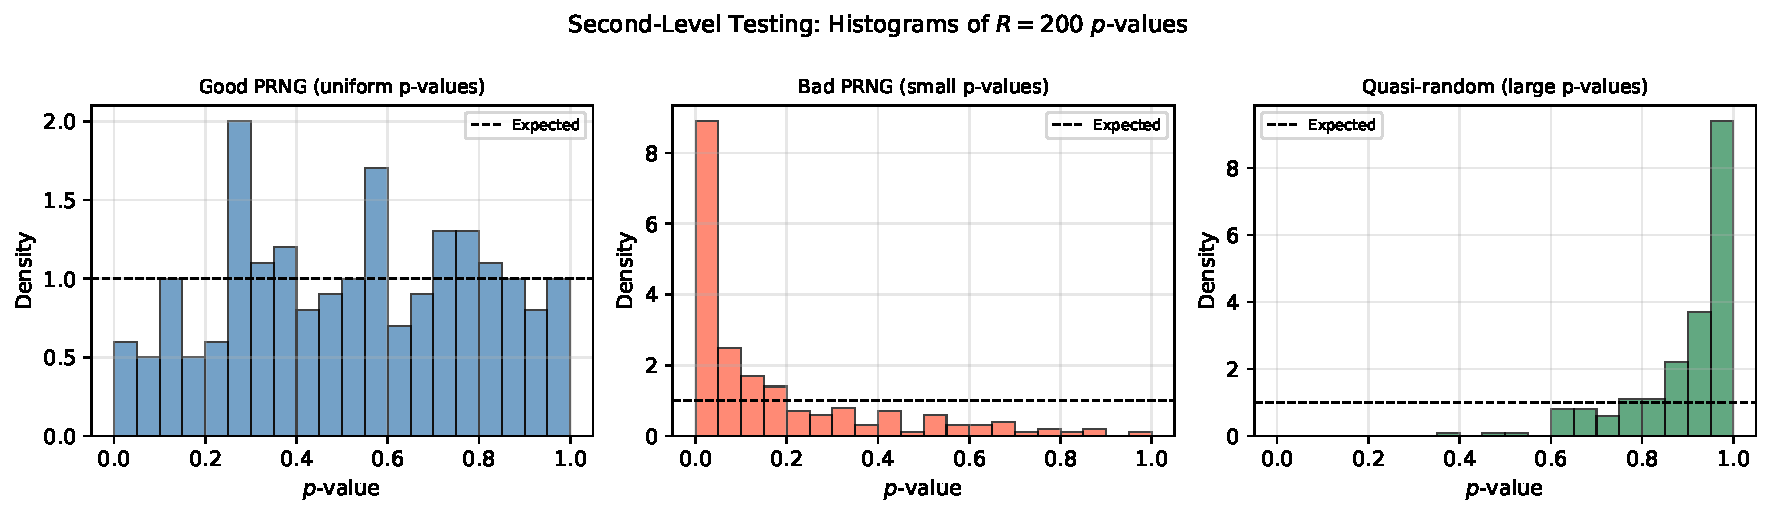
\includegraphics[width=0.76\textwidth]{second_level}
\end{center}

\framebreak

\textbf{Practical recommendations (NIST SP 800-22).}
The NIST standard recommends using $1000 \le R \le 10{,}000$ subsequences,
each of length $2^{20} \le n \le 2^{32}$.  Use significance level
$\alpha$ (alpha) in the range $[0.001, 0.01]$.

The \emph{empirical pass rate} is the fraction of subsequences whose first-level
$p$-value exceeds the threshold $\alpha$:
\[
  \hat{B}
  \;=\; \frac{1}{R}\sum_{i=1}^R \mathbf{1}\bigl[p^{(i)} > \alpha\bigr].
\]
Here $\hat{B}$ (B-hat, where the hat denotes ``estimated'') should be close
to $1 - \alpha$ (the theoretical fraction of sequences that pass).  The NIST
standard requires $\hat{B}$ to lie within three standard deviations of this
expected value:
\[
  \hat{B} \;\in\;
  \left[1 - \alpha \;\pm\; 3\sqrt{\frac{\alpha(1-\alpha)}{R}}\right].
\]

\begin{exampleblock}{Example 2.5.12: Second-Level KS Test on Sets A, B, C ($R=200$)}
Apply the KS test to $R = 200$ length-$n = 50$ subsequences:

\textbf{Set A (PCG64):} The 200 first-level $p$-values spread roughly
uniformly across $[0,1)$.  The second-level chi-square test gives a large
$p$-value (near 50\%), confirming that the first-level $p$-values look
uniform.  Set~A \textbf{passes}.

\textbf{Set B (biased):} Every subsequence exhibits the same leftward skew,
so every first-level $p$-value is small (near 0).  The histogram of $p$-values
is heavily concentrated at the left end.  The second-level chi-square statistic
is enormous and $p_{\mathrm{final}} \approx 0$.  Set~B \textbf{fails}.

\textbf{Set C (quasi-random):} Every subsequence is ``too uniform'', so
every first-level KS $p$-value is large (near 1.0).  The histogram is
concentrated at the right end.  The second-level chi-square statistic is
again enormous and $p_{\mathrm{final}} \approx 0$.  Set~C is
\textbf{detected as non-random}, even though the first-level KS test did
not reject it.
\end{exampleblock}

\begin{alertblock}{Key Insight: Second-Level Testing Is Essential}
Second-level testing is strictly more powerful than first-level testing
for detecting subtle non-randomness.  It is the \emph{only} reliable
method to detect quasi-random sequences that fool first-level tests by
being ``too uniform''.  It is also the primary defence against overfitting:
a generator whose parameters were tuned to pass one particular first-level
test will still fail the second-level test if its $p$-values cluster
near a single value rather than spreading uniformly across $[0,1)$.
\end{alertblock}

\end{frame}

%% ------------------------------------------------------------------
\begin{frame}[fragile]{2.5.6 Python Code: Second-Level Testing}

\begin{lstlisting}[style=python]
import numpy as np
from scipy import stats

def second_level_test(sequences, test_fn, s=10):
    """
    Apply test_fn to each sequence to obtain a first-level p-value.
    Then check whether those p-values are U[0,1) using a chi-square
    uniformity test with s equal bins.

    Parameters
    ----------
    sequences : list of 1D arrays   (each is one subsequence)
    test_fn   : callable returning a float p-value for one sequence
    s         : int, number of equal bins for the second-level test

    Returns
    -------
    p_vals    : array of first-level p-values (length R)
    chi2_stat : second-level chi-square statistic
    p_final   : second-level p-value (should be ~uniform if H0 true)
    """
    p_vals        = np.array([test_fn(seq) for seq in sequences])
    obs, _        = np.histogram(p_vals, bins=np.linspace(0, 1, s + 1))
    exp           = [len(p_vals) / s] * s
    chi2_stat, p_final = stats.chisquare(obs, exp)
    return p_vals, chi2_stat, p_final

# --- Set A: 200 PCG64 subsequences of length 50 --------------------
rng    = np.random.default_rng(0)
R, n   = 200, 50
seqs_A = [rng.random(n) for _ in range(R)]

# --- Set C: quasi-random shifted equispaced sequences ---------------
# Each subsequence is a shifted version of the uniform grid
seqs_C = [(np.arange(n) / n + i / R) % 1.0 for i in range(R)]

def ks_pval(seq):
    """First-level KS p-value for one sequence."""
    _, p = stats.kstest(seq, 'uniform')
    return p

pA, chi2_A, p2_A = second_level_test(seqs_A, ks_pval)
pC, chi2_C, p2_C = second_level_test(seqs_C, ks_pval)

print(f"2nd-level KS (Set A): chi2={chi2_A:.2f},  p={p2_A:.4f}")
print(f"2nd-level KS (Set C): chi2={chi2_C:.2f},  p={p2_C:.6f}")
# Expected output:
# Set A: small chi2, large p  -> passes (p-values are uniform)
# Set C: huge chi2, p ~ 0     -> fails  (p-values cluster near 1)
\end{lstlisting}

\end{frame}

%% ==================================================================
\begin{frame}[allowframebreaks]{2.6 Bibliographical Notes}

This chapter draws on five decades of PRNG research.  The references below
provide essential deeper reading for each major topic.

\medskip
\textbf{Foundational references on generators:}

\emph{Knuth} [107], \emph{The Art of Computer Programming, Volume~2:
Seminumerical Algorithms} (3rd ed., 1997): the definitive mathematical
treatment of LCGs.  Proves the full-period conditions (Theorem~2.4.1),
analyses the spectral test in detail, covers the Fibonacci and Lagged
Fibonacci generators, the serial test, and the poker test.  The most
comprehensive single reference on practical PRNG theory.

\emph{L'Ecuyer} [118, 122]: designed the combined generators described in
Section~2.4.1 and co-developed the TestU01 test suite with Simard.  His
combined GLCG paper (1988) introduced the principle of using multiple
generators with offset lattice structures to achieve very long effective
periods.  His TestU01 paper (2007) remains the benchmark reference for
PRNG testing: BigCrush comprises 106 statistical tests and requires
approximately $10^{10}$ random numbers to complete a single run.

\emph{Marsaglia} [141, 145]: invented the Diehard test battery (the first
systematic battery for testing PRNGs) and the birthday spacing test; his
1968 paper proved the lattice structure result that is now named Marsaglia's
theorem.  The Diehard battery was widely used through the 1990s and 2000s.

\emph{NIST SP 800-22} [187]: the US National Institute of Standards and
Technology statistical test suite for cryptographic PRNGs.  Contains 15
standardised tests including the monobit test, block frequency test, runs
test, and random excursion test.  Any generator used in a cryptographic
context should pass this suite as a minimum requirement.

\framebreak

\textbf{Modern generators:}

\emph{PCG64} (O'Neill [162]): Permuted Congruential Generators (2014).
The current NumPy default, accessible via \texttt{default\_rng}.  Uses a
128-bit LCG internal state with a nonlinear output permutation that
eliminates the lattice structure while maintaining a period of $2^{128}$.
Passes all TestU01 BigCrush tests.  Supports jumping ahead to arbitrary
positions, enabling multiple independent parallel streams.

\emph{MT19937} (Matsumoto and Nishimura [146], 1998): Mersenne Twister.
Period $2^{19937}-1$; state of 624 32-bit integers (2.5 KB).  Passes
Diehard but fails some TestU01 BigCrush tests.  Not suitable for
cryptographic use.  Was the NumPy default before PCG64 and is still the
default for Python's built-in \texttt{random} module.

\emph{AES-CTR and ChaCha20}: cryptographically secure stream ciphers that
have replaced RC4 in modern protocols (RFC~7539 and RFC~8439).  Both have
formal security proofs and are the recommended choices for any application
where the PRNG output must be computationally unpredictable.  ChaCha20 is
particularly attractive because it requires no special hardware support
and is resistant to timing side-channel attacks.

\medskip
\textbf{Shuffling and card mixing:}

\emph{Bayer and Diaconis} [14]: proved the ``7 shuffle theorem'' for the
riffle shuffle on 52 cards using Fourier analysis on the symmetric group
$\mathcal{S}_{52}$.  This 1992 paper introduced the ``cut-off phenomenon''
for card shuffling.

\emph{Aldous and Diaconis} [2]: Markov chain coupling methods for mixing-time
analysis; the theoretical foundation for Section~2.2.2.

\medskip
\textbf{Statistical tests and their mathematical foundations:}

\emph{Weiss} [210]: central limit theorem for the empty-boxes count
(Proposition~2.5.9).

\emph{Holst} [83] and \emph{L'Ecuyer et al.}\ [122]: known results on the
chi-square distribution of the serial test statistic.

\emph{Tsang et al.}\ [205]: analysis of the random excursion test including
the theoretical distribution of excursion visit counts.

\emph{L'Ecuyer and Simard} [169, 170]: design of reliable statistical tests
using Berry-Esseen bounds to control normal-approximation errors; explains
why TestU01 achieves precisely controlled Type I error rates.

\emph{Feller} [55], \emph{An Introduction to Probability Theory and Its
Applications, Volume~I}: classical reference for the arcsine law and other
random walk theorems used in Section~2.5.4.

\end{frame}

%% ==================================================================
\begin{frame}[allowframebreaks]{2.7 Selected Exercises}

The following exercises reinforce the theoretical foundations of this chapter.
Theoretical exercises are labelled ``T''; computational lab exercises are
labelled ``L''.

\medskip
\textbf{2.T.1 (Markov and Chebyshev Inequalities).}
Two fundamental inequalities bound the probability of large deviations.

For any \emph{non-negative} random variable $X$ (one that is always $\ge 0$)
and any constant $a > 0$, the \textbf{Markov inequality} states:
\[
  \mathbb{P}(X \;\ge\; a) \;\le\; \frac{\mathbb{E}X}{a}.
\]
Here $\mathbb{E}X$ (expected value of $X$) is the average of $X$ over all
possible outcomes, and $\mathbb{P}(X \ge a)$ is the probability that $X$
is at least as large as the threshold $a$.  The inequality says: the
probability of $X$ being very large is bounded by the ratio of its average
to that large value.

For a real-valued $X$ with finite variance $\mathrm{Var}X = \mathbb{E}[(X-\mathbb{E}X)^2]$
and any constant $b > 0$, the \textbf{Chebyshev inequality} states:
\[
  \mathbb{P}(|X - \mathbb{E}X| \;\ge\; b)
  \;\le\; \frac{\mathrm{Var}X}{b^2}.
\]
Here $|X - \mathbb{E}X|$ (the absolute value of $X$ minus its expected
value) measures how far $X$ is from its mean.  The Chebyshev inequality
follows from the Markov inequality applied to the non-negative variable
$(X - \mathbb{E}X)^2$: set $a = b^2$ in Markov to get
$\mathbb{P}((X - \mathbb{E}X)^2 \ge b^2) \le \mathrm{Var}X / b^2$.

\medskip
\textbf{2.T.4 (Integer Conversion).}
Let $U_1, U_2, \ldots$ be i.i.d.\ (independent and identically distributed)
$\mathcal{U}[0,1)$ and $M \ge 2$ an integer.  Show that the sequence
$Y_i = \lfloor M\,U_i \rfloor$ (floor of $M$ times $U_i$) consists of
i.i.d.\ uniformly distributed integers on $\{0, 1, \ldots, M-1\}$.

\emph{Hint:} compute $\mathbb{P}(Y_i = k) = \mathbb{P}(k/M \le U_i < (k+1)/M)$
using the definition of the uniform distribution.  This probability should
equal $1/M$ for every $k \in \{0, \ldots, M-1\}$, confirming that $Y_i$
is uniform on $\bar{M}$.

\framebreak

\textbf{2.T.8 (Correctness of Fisher-Yates).}
Verify that Algorithm~1 (Fisher-Yates shuffle) produces a uniformly random
permutation of $\{1, \ldots, n\}$.

\emph{Hint:} proceed by induction on the swap steps.  After step $i$
(processing position $i$), show that the element now in position $i$ is
uniformly distributed over the $i$ elements not yet placed in higher
positions.  A permutation is uniform if and only if each element is equally
likely to end up in each position, and the Fisher-Yates induction establishes
exactly this.

\medskip
\textbf{2.T.17 (Serial Test Mean).}
Let $O_i$ ($i = 1, \ldots, k$) be the number of random vectors
$\mathbf{u}_j$ falling into box $i$ in the serial test, where $r$ vectors
of dimension $m$ are thrown into $k = L^m$ boxes.  Show that under
$\mathcal{H}_0$: $\mathbb{E}[X_k^2] = k - 1$, where $X_k^2$ is the
chi-square statistic.

\emph{Hint:} expand $X_k^2 = \sum_{i=1}^k (O_i - r/k)^2 / (r/k)$,
compute $\mathbb{E}[O_i] = r/k$ and $\mathrm{Var}(O_i) = r(1-1/k)/k$
from the multinomial distribution, and sum across the $k$ bins.

\medskip
\textbf{2.T.19 (Riffle Shuffle and Time Reversal).}
Let $p_{\mathrm{RS}}(\sigma, \sigma')$ denote the one-step transition
probability of the Riffle Shuffle (from permutation $\sigma$ to $\sigma'$)
and $p_{\mathrm{TR-RS}}(\sigma, \sigma')$ the time-reversed Riffle Shuffle.
Show that $p_{\mathrm{RS}}(\sigma, \sigma') = p_{\mathrm{TR-RS}}(\sigma', \sigma)$
for any $\sigma, \sigma' \in \mathcal{S}_n$.  This means the Riffle Shuffle
and its time-reversed version are related by swapping the source and target
permutations --- a symmetry that simplifies the analysis of mixing times.

\framebreak

\textbf{Lab Exercises:}

\textbf{2.L.1 (LCG Period Verification).}
Implement the LCG with $M = 2^{11} - 1 = 2047$, $a = 5$, $c = 1$.
\begin{enumerate}[(a)]
  \item Generate $10^4$ output numbers and plot $(i, u_i)$ versus $i$
    (index on the $x$-axis, output on the $y$-axis).  Observe the
    periodic pattern.
  \item Find the period computationally by tracing the state sequence
    until a state repeats.
  \item Verify Theorem~2.4.1 by checking all three conditions for
    $(a, c, M) = (5, 1, 2047)$.
\end{enumerate}

\textbf{2.L.2 (Broken Fisher-Yates).}
Compare the correct Fisher-Yates algorithm (Algorithm~1) to a ``broken''
version in which line~3 is replaced by $k = \mathrm{random}(1, \ldots, n)$
(drawing the swap index uniformly from the \emph{full} range $\{1,\ldots,n\}$
rather than $\{1,\ldots,i\}$).
\begin{enumerate}[(a)]
  \item Generate $10^4$ permutations using each version.
  \item Apply the fixed-point permutation test (Section~2.5.5) to both.
  \item Explain why the broken version fails: enumerate the $3! = 6$
    permutations of $\{1,2,3\}$ reachable by the broken version and check
    that some are more likely than others.
\end{enumerate}

\textbf{2.L.3 (Autocorrelation Comparison).}
Generate $n = 10^5$ numbers from each of MT19937 and the LMCG with
$(M, a) = (2^{31}-1, 16{,}807)$.  Compute the Pearson autocorrelation
between $(y_1, \ldots, y_{n-1})$ and $(y_2, \ldots, y_n)$.  Which generator
shows less autocorrelation?  Compute the autocorrelation for lags 1, 2, 5,
and 10 and compare the results.

\textbf{2.L.5 (Quasi-Random Detection).}
Let $u_i = (i \cdot \phi) \bmod 1$ for $i = 1, \ldots, n = 10^6$, where
$\phi = (\sqrt{5}-1)/2 \approx 0.6180$ is the golden ratio (this is the
Kronecker low-discrepancy sequence).
\begin{enumerate}[(a)]
  \item Apply the KS test and report the $p$-value.
  \item Apply the chi-square test with 10 uniform bins and report the $p$-value.
  \item Apply the frequency of pairs test ($L = 10$, $r = 500{,}000$ pairs)
    and report the $p$-value.
  \item Apply second-level KS testing with $R = 1000$ subsequences of length
    $n/R = 1000$ each.  Report the second-level $p$-value.
  \item Observe that first-level tests pass (or produce a suspiciously high
    $p$-value) while second-level testing conclusively detects the
    quasi-randomness.
\end{enumerate}

\end{frame}

%% ==================================================================
\begin{frame}{Chapter 2: Summary}

\begin{columns}
\column{0.50\textwidth}
\textbf{Generators:}
\begin{itemize}
  \item A PRNG is a 5-tuple $(S, s_0, f, V, g)$; the period is at most $|S|$.
  \item Three equivalent sequence types: $\mathcal{U}[0,1)$, random bits,
    and uniform integers on $\{0,\ldots,M-1\}$.
  \item Fisher-Yates shuffle produces a uniform random permutation in
    $\mathcal{O}(n)$ time (optimal).
  \item The seven-shuffle theorem: 7 riffle shuffles suffice for 52 cards.
  \item Python: \texttt{default\_rng}/PCG64 (period $2^{128}$) and MT19937
    (period $2^{19937}-1$).
  \item RC4: KSA + PRGA permutation cipher; deprecated in 2015 (RFC~7465)
    due to key-correlated biases.
  \item LCG full-period conditions: $\gcd(c,M)=1$; every prime of $M$
    divides $a-1$; and $4 \mid M \Rightarrow 4 \mid (a-1)$.
  \item Marsaglia's theorem: all LCG $d$-tuples lie on at most $M^{1/d}$
    parallel hyperplanes.
  \item Bit generators: LFSR, XORG, SXR (fast non-cryptographic);
    BBS (provably secure but slow).
  \item L'Ecuyer combined generator: period $\approx 2^{191}$ from two
    components each with period $\approx 2^{32}$.
\end{itemize}

\column{0.50\textwidth}
\textbf{Statistical Testing:}
\begin{itemize}
  \item KS test: $D_n = \sup|\hat{F}_n(t) - t|$; detects 1D non-uniformity.
  \item Chi-square: $X^2 = \sum(O_i-E_i)^2/E_i$ with $E_i \ge 5$ per bin.
  \item Serial (pairs) test: detects 2D correlations invisible to 1D tests.
  \item Balls-and-boxes: birthday, collision, birthday spacing, poker ---
    all unified by multinomial occupancy theory.
  \item Random walk: monobit (global bit balance), block frequency (local
    balance), arcsine law (time above zero), random excursion (visit counts).
  \item Permutation: derangement count and fixed-point distribution, both
    with known exact theoretical distributions.
  \item Second-level testing: apply any test to $R \ge 1000$ subsequences;
    check that the resulting $p$-values are $\mathcal{U}[0,1)$.  The only
    reliable method to detect quasi-random sequences.
  \item A test can only \emph{reject}, never confirm; passing BigCrush is
    strong practical evidence but not a mathematical guarantee.
\end{itemize}
\end{columns}

\medskip
\begin{alertblock}{Take-Home Message}
No PRNG is universally perfect, but modern generators (PCG64) pass all
practical statistical tests and are the recommended choice for Monte Carlo
simulations.  Cryptographic applications additionally require computational
unpredictability: use AES-CTR or ChaCha20, not RC4.  Second-level testing
is the only reliable method to detect quasi-random sequences that fool
first-level tests by being ``too uniform''.  Always check your generator
with second-level testing before a long, expensive simulation.
\end{alertblock}

\end{frame}

\end{document}
